\documentclass{createspace}
\newcommand{\N}{\mathbb N}
\newcommand{\Z}{\mathbb Z}
\newcommand{\Q}{\mathbb Q}
\newcommand{\R}{\mathbb R}
\newcommand{\C}{\mathbb C}

\newcommand{\shrap}{\mathbin{\#}}
\DeclareMathOperator*{\bigshrap}{\#}

\newcommand{\bracket}[1]{\left\langle{#1}\right\rangle}

\newcommand{\alexander}{\Delta}
\newcommand{\conway}{\nabla}
\newcommand{\jones}{V}
% span?

\newcommand{\braid}{\operatorname{b}}
\newcommand{\bridge}{\operatorname{br}}
\newcommand{\crossing}{\operatorname{cr}}
\newcommand{\genus}{\operatorname{g}}
\newcommand{\linking}{\operatorname{lk}}
\newcommand{\sign}{\operatorname{sgn}}
\newcommand{\volume}{\operatorname{vol}}
\newcommand{\writhe}{\operatorname{wr}}

\newcommand{\MalyNieWezel} {\begin{tikzpicture}[baseline=-0.65ex, scale=0.02]
	\begin{knot}[clip width=5, end tolerance=1pt]
		\strand[semithick] (0,0) circle (5);
	\end{knot}
\end{tikzpicture}}

\newcommand{\NieWezel} {\begin{tikzpicture}[baseline=-0.65ex, scale=0.04]
	\begin{knot}[clip width=5, end tolerance=1pt]
		\strand[semithick] (0,0) circle (5);
	\end{knot}
\end{tikzpicture}}

\newcommand{\PrawyKrzyz} {\begin{tikzpicture}[baseline=-0.65ex, scale=0.04]
	\useasboundingbox (-5, -5) rectangle (5,5);
	\begin{knot}[clip width=5, end tolerance=1pt, flip crossing/.list={1}] 
		\strand[semithick] (-5,5) to (5,-5);
		\strand[semithick] (-5,-5) to (5,5);
	\end{knot}
\end{tikzpicture}}

\newcommand{\MalyPrawyGladki} {
	\begin{tikzpicture}[baseline=-0.65ex,scale=0.03]
	\begin{knot}[clip width=5, end tolerance=1pt] 
		\strand[semithick] (-4, -5) to [out=45, in=-45] (-4, 5);
		\strand[semithick] (4, -5) to [out=135, in=-135] (4, 5);
	\end{knot}
	\end{tikzpicture}
}

\newcommand{\MalyPrawyKrzyz} {\begin{tikzpicture}[baseline=-0.65ex, scale=0.03]
	\useasboundingbox (-5, -5) rectangle (5,5);
	\begin{knot}[clip width=5, end tolerance=1pt, flip crossing/.list={1}] 
		\strand[semithick] (-5,5) to (5,-5);
		\strand[semithick] (-5,-5) to (5,5);
	\end{knot}
\end{tikzpicture}}

\newcommand{\PrawyGladkiKreslony} {
	\begin{tikzpicture}[baseline=-0.65ex,yscale=0.07, xscale=0.1]
	\useasboundingbox (-5, -6) rectangle (5, 6);
	\begin{knot}[clip width=5, end tolerance=1pt] 
		\strand[semithick] (-4, -5) to [out=45, in=-45] (-4, 5);
		\strand[semithick] (4, -5) to [out=135, in=-135] (4, 5);
		\strand[semithick] (-5, 0) to (5, 0);
	\end{knot}
	\end{tikzpicture}
}

\newcommand{\LewyGladkiKreslony} {
	\begin{tikzpicture}[baseline=-0.65ex,yscale=0.07, xscale=0.1]
	\useasboundingbox (-5, -6) rectangle (5, 6);
	\begin{knot}[clip width=5, end tolerance=1pt] 
		\strand[semithick] (-5, 5) [in=-135, out=-45] to (5,5);
		\strand[semithick] (-5, -5) [in=135, out=45] to (5,-5);
		\strand[semithick] (-5, 0) to (5, 0);
	\end{knot}
	\end{tikzpicture}
}

\newcommand{\LewyKrzyz} {\begin{tikzpicture}[scale=0.03, baseline=-3]
	\begin{knot}[clip width=5, end tolerance=1pt] 
		\strand[semithick] (-5,5) to (5,-5);
		\strand[semithick] (-5,-5) to (5,5);
	\end{knot}
\end{tikzpicture}}

\newcommand{\MalyLewyGladki} {
	\begin{tikzpicture}[baseline=-0.65ex,scale=0.03]
	\begin{knot}[clip width=5, end tolerance=1pt] 
		\strand[semithick] (-5, 5) [in=-135, out=-45] to (5,5);
		\strand[semithick] (-5, -5) [in=135, out=45] to (5,-5);
	\end{knot}
	\end{tikzpicture}
}

\newcommand{\MalyLewyKrzyz} {
	\begin{tikzpicture}[baseline=-0.65ex,scale=0.03]
	\begin{knot}[clip width=5, end tolerance=1pt] 
		\strand[semithick] (-5, -5) to [out=up, in=up] (5, -5);
		\strand[semithick] (-5, 5) to [out=down, in=down] (5, 5);
	\end{knot}
	\end{tikzpicture}
}

\newcommand{\reidemeisterIa} {
\begin{tikzpicture}[baseline=-0.65ex, scale=0.07]
\useasboundingbox (-4, -5) rectangle (3, 5);
\begin{knot}[clip width=5, end tolerance=1pt] 
	\strand[semithick] (-3,  5) [in=left, out=down] to (1, -2) [in=down, out=right] to (3, 0);
	\strand[semithick] (-3, -5) [in=left, out=up]   to (1,  2) [in=up,   out=right] to (3, 0);
\end{knot}
\end{tikzpicture}
}

\newcommand{\MalyreidemeisterIa} {\begin{tikzpicture}[baseline=-0.65ex, scale=0.03]
\useasboundingbox (-4, -5) rectangle (3, 5);
\begin{knot}[clip width=5, end tolerance=1pt] 
	\strand[semithick] (-3,  5) [in=left, out=down] to (1, -2) [in=down, out=right] to (3, 0);
	\strand[semithick] (-3, -5) [in=left, out=up]   to (1,  2) [in=up,   out=right] to (3, 0);
	\end{knot}
	\end{tikzpicture}}

\newcommand{\MalyreidemeisterIb} {\begin{tikzpicture}[baseline=-0.65ex, scale=0.03]
	\begin{knot}[clip width=5, end tolerance=1pt] 
		\strand[semithick] (0,-5) to (0, 5);
	\end{knot}
\end{tikzpicture}}

\newcommand{\reidemeisterIb} {
\begin{tikzpicture}[baseline=-0.65ex, scale=0.07]
\begin{knot}[clip width=5, end tolerance=1pt] 
	\strand[semithick] (0,-5) to (0, 5);
\end{knot}
\end{tikzpicture}
}

% potrzebne do klamry Kauffmana
\newcommand{\reidemeisterIab} {
\begin{tikzpicture}[baseline=-0.65ex,scale=0.07]
\useasboundingbox (-5, -6) rectangle (5, 6);
\begin{knot}[clip width=5, end tolerance=1pt] 
	\strand[semithick] (4,-5) .. controls (4,-3) and (-4,-3) .. (-4,-1);
	\strand[semithick] (-4,-5) .. controls (-4,-3) and (4,-3) .. (4,-1);
	\strand[semithick] (-4,-1) [in=left, out=up] to (0, 1) to [in=up, out=right] (4,-1);
	\strand[semithick] (-4, 5) [in=left, out=down] to (0, 3) to [in=down, out=right] (4, 5);
\end{knot}
\end{tikzpicture}
}

\newcommand{\reidemeisterIIa} {
\begin{tikzpicture}[baseline=-0.65ex,scale=0.07]
\useasboundingbox (-5, -6) rectangle (5, 6);
\begin{knot}[clip width=5, end tolerance=1pt] 
	\strand[semithick] (4,-5) .. controls (4,-2) and (-4,-2) .. (-4,0);
	\strand[semithick] (4,5) .. controls (4, 2) and (-4, 2) .. (-4,0);
	\strand[semithick] (-4,-5) .. controls (-4,-2) and (4,-2) .. (4,0);
	\strand[semithick] (-4,5) .. controls (-4, 2) and (4,2) .. (4,0);
\end{knot}
\end{tikzpicture}
}

% reidemeister II a poziomo
\newcommand{\reidemeisterIIaa} {
\begin{tikzpicture}[baseline=-0.65ex,scale=0.05]
\begin{knot}[clip width=5, end tolerance=1pt] 
	\strand[semithick] (-10, -5) to [out=right, in=left] ( 0,  5) 
	                             to [out=right, in=left] (10, -5);
	\strand[semithick] (-10,  5) to [out=right, in=left] ( 0, -5) 
	                             to [out=right, in=left] (10,  5);
\end{knot}
\end{tikzpicture}
}

\newcommand{\reidemeisterIIb} {
\begin{tikzpicture}[baseline=-0.65ex,scale=0.07]
\begin{knot}[clip width=5, end tolerance=1pt] 
	\strand[semithick] (4,-5) .. controls (4,-2) and (1,-2) .. (1,0);
	\strand[semithick] (4,5) .. controls (4, 2) and (1, 2) .. (1,0);
	\strand[semithick] (-4,-5) .. controls (-4,-2) and (-1,-2) .. (-1,0);
	\strand[semithick] (-4,5) .. controls (-4, 2) and (-1,2) .. (-1,0);
\end{knot}
\end{tikzpicture}
}

\newcommand{\reidemeisterIIIa} {
\begin{tikzpicture}[baseline=-0.65ex,yscale=0.07, xscale=0.1]
\useasboundingbox (-5, -6) rectangle (5, 6);
\begin{knot}[clip width=5, flip crossing/.list={1,2,3}, end tolerance=1pt] 
	\strand[semithick] (-5,-5) -- (5,5);
	\strand[semithick] (-5,5) -- (5,-5);
	\strand[semithick] (-5,-1) .. controls (-2, -1) and (-2,4) .. (0,4) .. controls (2, 4) and (2, -1) .. (5, -1);
\end{knot}
\end{tikzpicture}
}

\newcommand{\reidemeisterIIIb} {
\begin{tikzpicture}[baseline=-0.65ex,yscale=0.07, xscale=0.1]
\useasboundingbox (-5, -6) rectangle (5, 6);
\begin{knot}[clip width=5, flip crossing/.list={1,2,3}, end tolerance=1pt] 
	\strand[semithick] (-5,-5) -- (5,5);
	\strand[semithick] (-5,5) -- (5,-5);
	\strand[semithick](-5,+1) .. controls (-2,+1) and (-2,-4) .. (0,-4) .. controls (2,-4) and (2,+1) .. (5,+1);
\end{knot}
\end{tikzpicture}
}

\newcommand{\skeinplus} {
\begin{tikzpicture}[baseline=-0.65ex,scale=0.1]
\useasboundingbox (-5, -6) rectangle (5, 6);
\begin{knot}[clip width=5, end tolerance=1pt] 
	\strand[semithick,-latex] (-5, -5) to (5,  5);
	\strand[semithick,latex-] (-5,  5) to (5, -5);
	\node[darkblue] at (0,-4)[below] {$L_+$};
\end{knot}
\end{tikzpicture}
}

\newcommand{\skeinminus} {
\begin{tikzpicture}[baseline=-0.65ex,scale=0.1]
\useasboundingbox (-5, -6) rectangle (5, 6);
\begin{knot}[clip width=5, end tolerance=1pt, flip crossing/.list={1}] 
	\strand[semithick,-latex] (-5, -5) to (5,  5);
	\strand[semithick,latex-] (-5,  5) to (5, -5);
	\node[darkblue] at (0,-4)[below] {$L_-$};
\end{knot}
\end{tikzpicture}
}

\newcommand{\skeinzero} {
\begin{tikzpicture}[baseline=-0.65ex,scale=0.1]
\useasboundingbox (-5, -6) rectangle (5, 6);
\begin{knot}[clip width=5, end tolerance=1pt, flip crossing/.list={1}] 
	\strand[semithick,-latex] (-5, -5) to [out=45, in=-45] (-5, 5);
	\strand[semithick,-Latex] (5, -5) to [out=135, in=-135] (5, 5);
	\node[darkblue] at (0,-4)[below] {$L_0$};
\end{knot}
\end{tikzpicture}
}

\tikzset{
	->-/.style={decoration={markings, mark=at position .5 with {\arrow{>}}},postaction={decorate}},
	-<-/.style={decoration={markings, mark=at position .5 with {\arrow{<}}},postaction={decorate}},
	LUK/.style ={
		draw=black,
		line join=miter,
		line cap=butt,
		miter limit=4.00,
		line width=0.2 mm
	},
	CIENKILUK/.style ={
		draw=black,
		line join=miter,
		line cap=butt,
		miter limit=4.00,
		line width=0.1 mm
	},
	TEKSTOWY/.style ={
		draw=black,
		line join=round,
		line cap=butt,
		miter limit=20.00,
		line width=0.2 mm
	},
	OBSZAR/.style={
		draw=none,
		fill=white!#1!red
	},
	OBSZAR/.default = 80,
}

\usepackage{enumitem}
\usepackage{booktabs}
\usepackage{longtable}
\usepackage[table]{xcolor}
\usepackage[colorinlistoftodos,prependcaption]{todonotes}
\usepackage{tikz}
\usetikzlibrary{arrows.meta}
\usetikzlibrary{decorations.markings}
\usetikzlibrary{decorations.pathreplacing}
\usetikzlibrary{knots}
\colorlet{darkblue}{blue!80!black}

\author{Leon Suwalski}
\title{Krótkie wprowadzenie do teorii węzłów}
\date{2018}

\begin{document}
\maketitle
\tableofcontents
\chapter{Preludium}
\label{cha:preludium}
Teoria węzłów to gałąź topologii,
która powstała z~inspiracji węzłami,
jakie pojawiają się w~codziennym życiu: przy wiązaniu butów albo cumowaniu statków.
Zajmuje się ona badaniem przede wszystkim węzłów,
czyli pewnych włożeń okręgu $S^1$ w~trójwymiarową przestrzeń euklidesową $\R^3$ lub sferę $S^3$,
ale także splotów (zaplątanych w~sobie węzłów), warkoczy, supłów oraz podobnych obiektów.
Matematyczne węzły różnią się tym od zwykłych, że ich końce są ze sobą połączone.

Oto kilka przykładów.
Węzeł (a) nazywamy niewęzłem, jest to kalka angielskiego \emph{unknot}.
Następne w~kolejce widoczne są trójlistnik (b,~\emph{trefoil}), ósemka (c,~\emph{figure-eight}), pięciolistnik (d,~\emph{cinquefoil}) oraz słynna para Perko (e,~f~wg oryginalnej numeracji Rolfsena).
Pod diagramami umieściliśmy notację Alexandera-Briggsa, jeszcze do niej wrócimy.

\begin{figure}[H]
    \centering
    \begin{minipage}[b]{.14\linewidth}
        \centering
        $\begin{tikzpicture}[baseline=-0.65ex, scale=0.5] \begin{knot}[clip width=5, end tolerance=1pt] \strand[semithick] (0,0) circle (\linewidth); \end{knot}
\end{tikzpicture}$
        \subcaption{}
    \end{minipage}
    \begin{minipage}[b]{.14\linewidth}
        \centering
        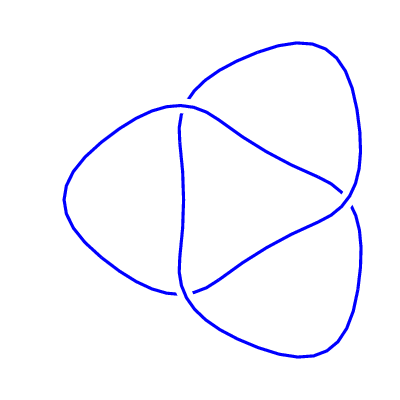
\includegraphics[width=\linewidth]{../data/3_1.png}
        \subcaption{$3_1$}
    \end{minipage}
    \begin{minipage}[b]{.14\linewidth}
        \centering
        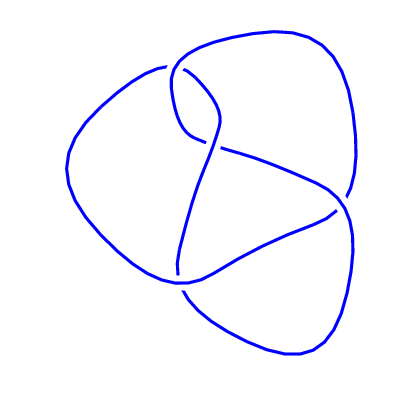
\includegraphics[width=\linewidth]{../data/4_1.png}
        \subcaption{$4_1$}
    \end{minipage}
    \begin{minipage}[b]{.14\linewidth}
        \centering
        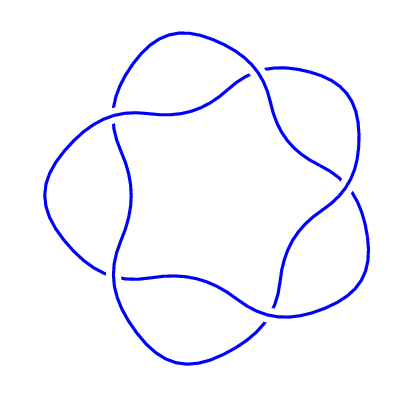
\includegraphics[width=\linewidth]{../data/5_1.png}
        \subcaption{$5_1$}
    \end{minipage}
    \begin{minipage}[b]{.14\linewidth}
        \centering
        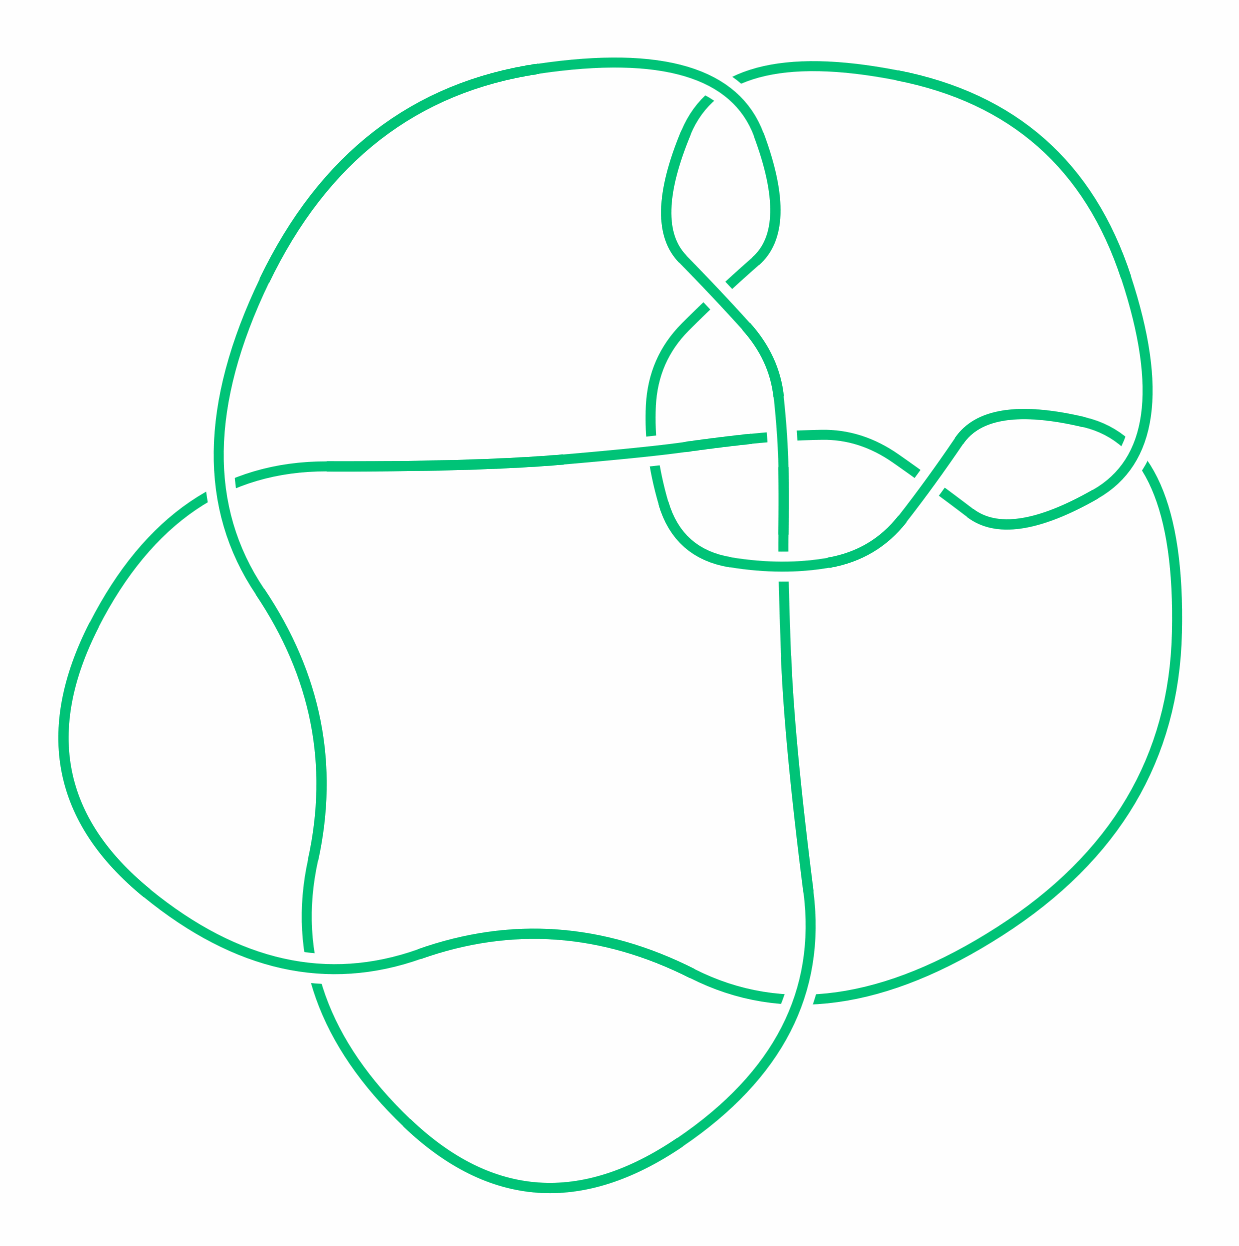
\includegraphics[width=\linewidth]{../data/perko1.png}
        \subcaption{$10_{161}$}
    \end{minipage}
    \begin{minipage}[b]{.14\linewidth}
        \centering
        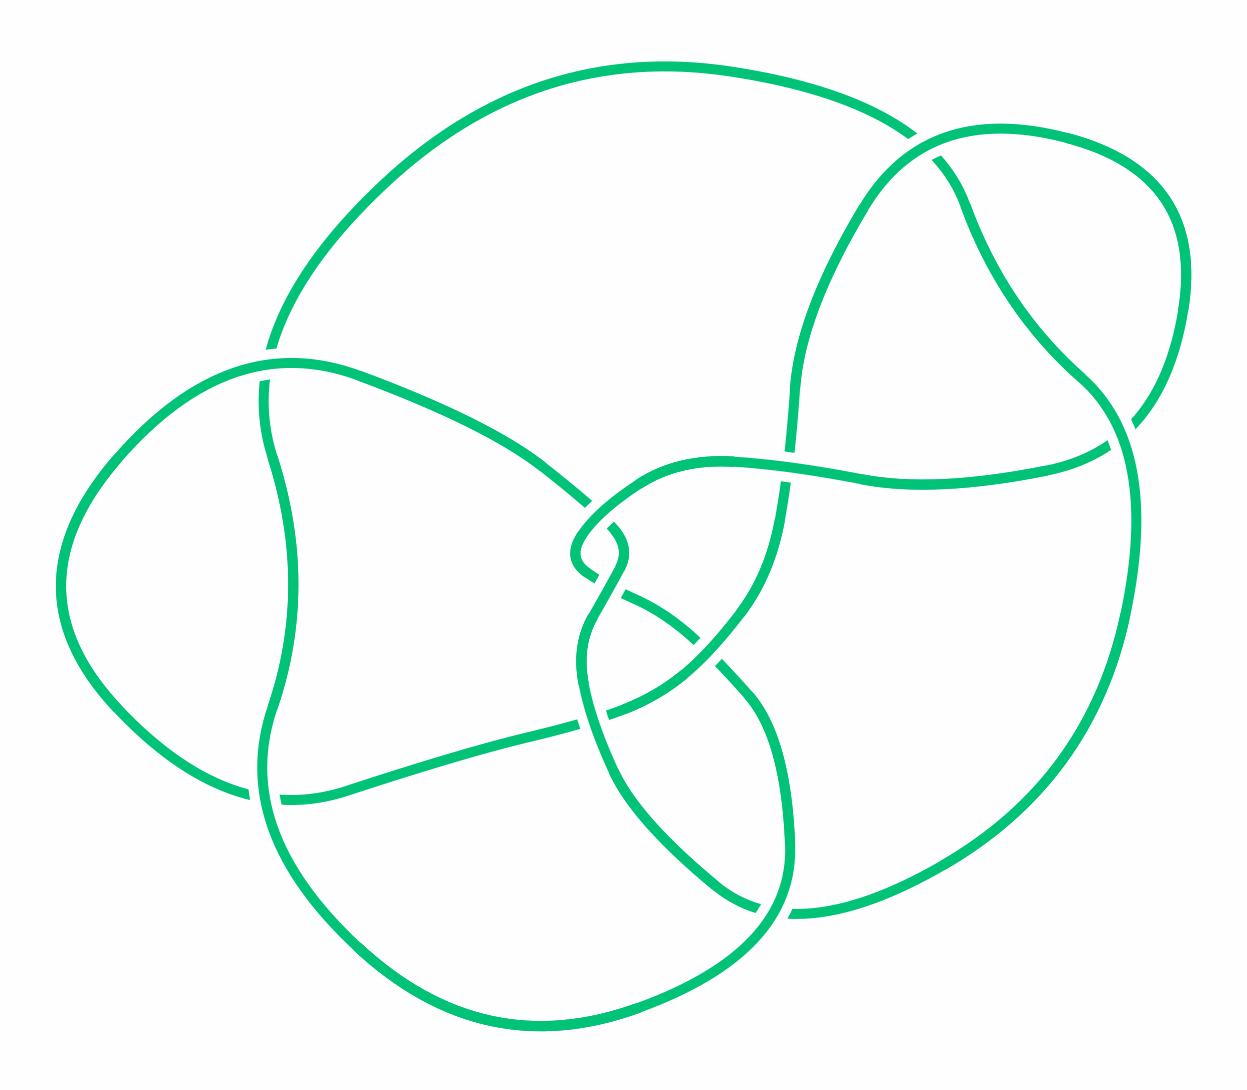
\includegraphics[width=\linewidth]{../data/perko2.png}
        \subcaption{$10_{162}$}
    \end{minipage}
\end{figure}

Początkowo celem teorii węzłów była klasyfikacja wszystkich węzłów.
Od XIX wieku, kiedy teoria węzłów wyodrębniła się jako osobny dział matematyki,
zdążyliśmy skatalogować ponad sześć miliardów tych obiektów.
Pozornie tak samo wyglądające węzły mogą się od siebie różnić.
Do wykrywania tych subtelnych różnic używa się przede wszystkim niezmienników topologicznych takich jak grupy, wielomiany bądź liczby.
Poznamy je w~dalszych rozdziałach.

Matematycy uogólnili pojęcie węzła:
można rozpatrywać je w~wyższych wymiarach albo zastąpić okrąg inną przestrzenią topologiczną.
Będziemy starać się unikać tych uogólnień.

\section{Węzły i~sploty}
Największą różnicą między węzłami matematycznymi oraz tymi z~prawdziwego jest życia jest to, że te pierwsze nie mają luźnych końców.
Można przyjąć nieidealną, naiwną definicję:

\begin{definition}[węzeł]
    Ciągłe oraz różnowartościowe odwzorowanie $S^1 \to \R^3$ nazywamy węzłem.
\end{definition}

Niestety, dopuszcza ona patologiczne z~kombinatorycznego punktu widzenia węzły dzikie, jak ten z~rysunku \ref{wild_knot}:

\begin{figure}
    \centering
    \label{wild_knot}
    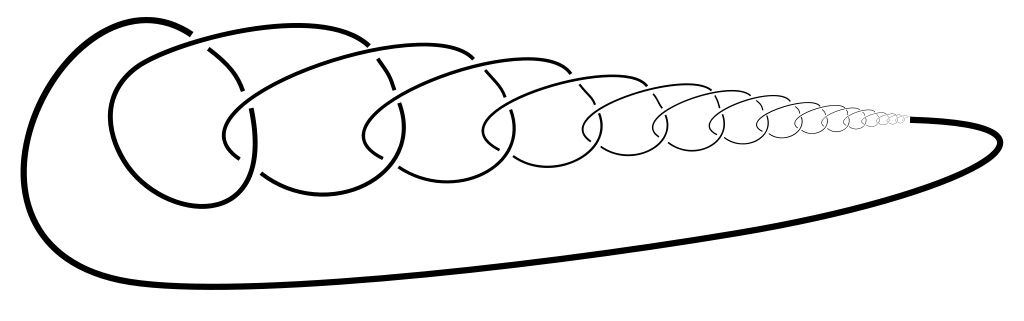
\includegraphics[width=0.5\linewidth]{wild_knot.png}
    \caption{Węzeł dziki}
\end{figure}

Zastanówmy się, jakim formalizmem opisać manipulowanie fizycznym sznurkiem, by wykluczyć węzły dzikie z~naszych rozważań.
Nie można użyć izotopii (dwa węzły są izotopijne, jeśli istnieje ciągła funkcja $F \colon S^1 \times [0, 1] \to \R^3$ taka, że $F(-, 0)$ jest pierwszym, zaś $F(-,1)$ drugim węzłem), gdyż każdy węzeł jest izotopijny z punktem:

{\color{red}\textbf{Tu brakuje obrazka.}}

W podobny sposób moglibyśmy przekształcić dowolny węzeł w~niewęzeł.
Teoria, w~której wszystkie obiekty są takie same, nie jest zbyt ciekawa.
Zwykła izotopia nie oddaje dobrze tego, czym jest równoważność węzłów wykonanych z~prawdziwego sznurka.
Trzeba od niej wymagać dodatkowo, by była gładka albo lokalnie płaska.
Z twierdzenia o rozszerzaniu izotopii wynika, że można ją wtedy podnieść do izotopii otaczającej.
Ta ostatnia uwzględnia, jak węzeł leży w~przestrzeni i okazuje się być właściwym pojęciem równości dla teorii węzłów:

\begin{definition}[izotopia otaczająca] \label{def_ambient_isotopy}
    Niech $N, M$ będą rozmaitościami, zaś $K_1, K_2 \colon N \to M$ włożeniami.
    Ciągłe odwzorowanie $F \colon M \times [0,1] \to M$ spełniające następujące warunki:
    \begin{enumerate}
        \item funkcja $F(-, 0)$ jest odwzorowaniem tożsamościowym,
        \item każda z funkcji $F(-, t)$ jest homeomorfizmem,
        \item złożenie $F(-, 1)$ z pierwszym włożeniem $K_1$ daje drugie włożenie $K_2$
    \end{enumerate}
    nazywamy izotopią otaczającą przenoszącą $K_1$ na $K_2$.
\end{definition}

W topologii rozważa się włożenia dowolnych rozmaitości, nam wystarczy jeden szczególny przypadek $N = S^1$ oraz $M = \R^3$.
Intuicyjnie, funkcja $F$ zniekształca przestrzeń $\R^3$ tak, że w~chwili początkowej $t = 0$ widzimy pierwszy, zaś w~chwili końcowej $t = 1$ drugi węzeł.
Izotopia otaczająca nie pozwala na ściąganie zaplątanych fragmentów do punktu.

{\color{red}\textbf{Homeomorfizmy $F_t$ można zastąpić przez dyfeomorfizmy zachowujące orientację. ???}}

\begin{definition}[węzeł]
    \label{def:knot}
    \index{węzeł}
    Gładkie włożenie $S^1 \to \R^3$ otaczająco izotopijne z~zamkniętą łamaną bez samoprzecięć nazywamy węzłem poskromionym.
\end{definition}

Przez prawie całą książkę interesować nas będą jedynie węzły poskromione,
dlatego jeśli nie zaznaczono inaczej, przez węzeł rozumiemy węzeł poskromiony.
Istnieje jeszcze jedna, konkurencyjna definicja węzłów równoważnych:

\begin{proposition}
    \label{equivalent_knots_2}
    Dwa węzły są równoważne, gdy jeden z~nich jest obrazem drugiego przez zachowujący orientację homeomorfizm $\R^3 \to \R^3$.
\end{proposition}

Stwierdzenie to przestaje być prawdziwe po zastąpieniu przestrzeni $\R^m$ przez $S^m$.

\begin{proof}
    Podany niżej dowód pochodzi z~książki ,,Topology from the differentiable viewpoint'' Johna Milnora.
    Musimy pokazać, że dyfeomorfizm $f \colon \R^m \to \R^m$ jest gładko izotopijny z~identycznością.
    Translacje są izotopiami, więc bez straty ogólności zakładamy, że $f(0) = 0$.
    Pochodna $f$ w~zerze jest dana wzorem $\mathrm{d}f_0(x) = \lim_{t \to 0} f(tx) /t$,
    naturalną definicję izotopii $F \colon \R^m \times [0, 1] \to \R^m$ stanowi więc
    \[
        F(x, t) = \begin{cases}
            \mathrm{d}f_0(x) & t = 0 \\
            f(tx) / t & 0 < t \le 1
        \end{cases} .
    \]

    Funkcja $F$ jest gładka, gdyż na mocy lematu Hadamarda funkcja $f$ zapisuje się jako suma $x_1 g_1(x) + \ldots + x_mg_m(x)$,gdzie funkcje $g_i$ są gładkie, co jakoś kończy dowód.
\end{proof}

Formalnie węzły to pewne odwzorowania, więc prawidłowym sposobem na zapisanie, że są izotopijne (czyli dla nas: równe), jest $K_1 \simeq K_2$.
Ponieważ nie prowadzi to do problemów, będziemy jednak stosować zapis $K_1 = K_2$.
Jednocześnie często węzeł (jako odwzorowanie) nie będzie odróżniany od obrazu tego odwzorowania.

\begin{definition}[splot, ogniwo]
    \label{def_link}
    \index{splot}
    Sumę parami rozłącznych węzłów $K_1, K_2, \ldots, K_n$ nazywamy splotem.
    Składniki sumy nazywamy ogniwami.
\end{definition}

Przez analogię do węzłów mówimy, że dwa sploty są takie same, jeśli jeden jest obrazem drugiego przez zachowujący orientację homeomorfizm $\R^3 \to \R^3$.
W~takiej sytuacji obydwa sploty mają tyle samo ogniw.

\begin{example}
    \index{splot!Hopfa}
    Splot Hopfa to najprostszy splot nietrywialny, którym w~1931 r. zajmował się Heinz Hopf, topolog niemiecki, w~ramach badań nad tzw. rozwłóknieniem (Hopf fibration).
    Whitehead w~1934 odkrył kontrprzykład do nieudanego dowodu hipotezy Poincarego.
    Był nim splot o~dwóch składowych przedstawiony na poniższym rysunku.

    \begin{figure}[H]
        \begin{minipage}[b]{.48\linewidth}
            \centering
            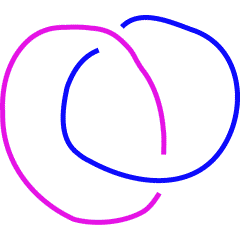
\includegraphics[width=0.5\linewidth]{../data/mixed/L2a1.png}
            \subcaption{splot Hopfa}
        \end{minipage}
        \begin{minipage}[b]{.48\linewidth}
            \centering
            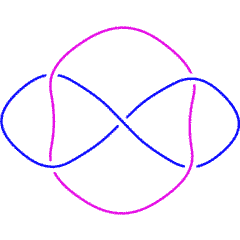
\includegraphics[width=0.5\linewidth]{../data/mixed/L5a1.png}
            \subcaption{splot Whiteheada}
        \end{minipage}
    \end{figure}
\end{example}

Jeśli dwa węzły są równoważne, to ich dopełnienia są oczywiście homeomorficzne.
Pytanie o~prawdziwość implikacji odwrotnej jako pierwszy zadał najprawdopodobniej w~1908 roku Tietze (,,Über die topologischen Invarianten mehrdimensionaler Mannigfaltigkeiten'').
W roku 1987 pokazano, że istnieją co najwyżej dwa węzły o~zadanym dopełnieniu (\cite{culler87}).
Dwa lata później poznaliśmy pozytywną odpowiedź na pytanie Tietzego: każdy węzeł jest wyznaczony jednoznacznie przez swoje dopełnienie.

\begin{theorem}[Gordon, Luecke, 1989]
    \label{thm_gordon_luecke}
    \index{twierdzenie!Gordona-Lueckego}
    Poskromione węzły o~homeomorficznych (z zachowaniem orientacji) dopełnieniach są wzajemnie izotopijne.
\end{theorem}

\begin{proof}[Niedowód]
    Wynika to z~ogólniejszego stwierdzenia:
    nietrywialna chirurgia Dehna na węźle w~3-sferze nigdy nie daje 3-sfery.
    Pełny dowód zawiera praca \cite{gordon89}.
\end{proof}

Twierdzenie to zamienia problem lokalny (czy dwa węzły w kuli $S^3$ są równoważne?) w~problem globalny (czy dwie przestrzenie topologiczne są homeomorficzne?).
Whitehead w~pracy \cite{whitehead37} z~1937 roku podał nieskończenie wiele splotów, których dopełnienia wyglądają jak dopełnienia splotu Whiteheada.
Odpowiednik twierdzenia \ref{thm_gordon_luecke} dla splotów jest więc fałszywy.

Poniższa definicja nie jest nam jeszcze potrzebna, ale wygodnie przytoczyć ją już teraz.

\begin{definition}[rozszczepialność]
    \index{splot!rozszczepialny}
    Jeżeli splot $L$ można zanurzyć w przestrzeni $\R^3$ tak, że niektóre jego ogniwa będą leżeć nad pewną rozłączną ze splotem płaszczyzną, zaś pozostałe pod nią, to powiemy, że splot $L$ jest rozszczepialny.
\end{definition}

Liczbę nierozszczepialnych splotów, pierwszych lub złożonych, zebrano w tabeli.
Źródło: baza danych OEIS, ciąg \href{https://oeis.org/A086825}{A086825}.

\renewcommand*{\arraystretch}{1.4}
\footnotesize
\begin{longtable}{lccccccccc}
    \hline
    \textbf{skrzyżowania}  &  0  &  1  &  2  &  3  &  4  &  5  &  6   &  7   &  8   \\  \hline  \endhead
    sploty                 &  1  &  0  &  1  &  1  &  3  &  4  &  15  &  24  &  82  \\
    \hline
\end{longtable}
\normalsize

\section{Diagramy. Ruchy Reidemeistera}
Chociaż w~świetle definicji \ref{def:knot} węzły są pewnymi regularnymi podzbiorami przestrzeni $\R^3$,
z kombinatorycznego punktu widzenia wygodniej jest rysować je na płaszczyźnie.

\begin{definition}[orientacja]
    \index{węzeł!zorientowany}
    Węzeł, w~którym wybrano kierunek, w~którym należy się po nim poruszać, nazywamy zorientowanym.
\end{definition}

\begin{definition} [diagram] \label{def_diagrams}
    \index{diagram}
    Cień to rzut węzła $K \subseteq \R^3$ na płaszczyznę.
    Cień razem z~informacją o~tym, jak przebiegają skrzyżowania i pozbawiony katastrof: potrójnych przecięć, stycznych czy dziobów nazywamy diagramem.
\end{definition}

{\color{red}\textbf{Narysować katastrofy}}

\begin{definition} [włókno]
    \index{włókno}
    Fragment diagramu, który biegnie między dwoma kolejnymi tunelami, czyli podskrzyżowaniami, nazywamy włóknem.
\end{definition}

\begin{definition} [nić]
    \index{nić}
    Fragment diagramu, który biegnie między dwoma kolejnymi skrzyżowaniami nazywamy nicią.
\end{definition}

Nici powstają z włókien przez rozcięcie ich przy każdym nadskrzyżowaniu.

\begin{proposition}
    Niech $K$ będzie węzłem.
    Zbiór diagramów jest otwarty i~gęsty w~zbiorze wszystkich rzutów.
\end{proposition}

\begin{proof}
    Rzut splotu na równoległe płaszczyzny jest taki sam, a te można sparametryzować prostymi przechodzącymi przez początek układu współrzędnych, które tworzą przestrzeń rzutową $\R \mathbb P^2$.
    Niech $S$ będzie zbiorem prostych, które dają złe rzuty.
    Wystarczy pokazać jego nigdziegęstość.
    Okazuje się, że $S$ jest też jednowymiarowy.
    (Dowód za \cite{crowell63}).
\end{proof}

Wynika stąd, że każdy węzeł ma wiele diagramów.
Mając dane dwa różne diagramy chcielibyśmy wiedzieć, czy reprezentują ten sam węzeł.
Na szczęście Reidemeister w latach 20. XX wieku podał proste kryterium rozstrzygające ten problem.
Najpierw zdefiniujmy trzy lokalne operacje na diagramach.

\begin{definition}
    \index{ruchy Reidemeistera}
    Trzy ruchy Reidemeistera, $R_1$, $R_2$, oraz $R_3$, to następujące deformacje diagramu:
    \[
        \underbrace{\begin{tikzpicture}[baseline=-0.65ex,scale=0.1]
        \begin{knot}[clip width=5]
            \strand[thick] (-5, 10) to [in=left, out=down] (2, -5);
            \strand[thick] (5, 0) to [in=right, out=down] (2, -5);
            \strand[thick] (5, 0) to [in=right, out=up] (2, 5);
            \strand[thick] (-5, -10) to [in=left, out=up] (2, 5);
        \end{knot}
        \end{tikzpicture}
        \, \cong \,
        \begin{tikzpicture}[baseline=-0.65ex,scale=0.1]
        \begin{knot}[clip width=5]
            \strand[thick] (0,10) to (0,-10);
        \end{knot}
        \end{tikzpicture}}_{R_1}
        %%%
        \quad \quad \quad
        \underbrace{\begin{tikzpicture}[baseline=-0.65ex,scale=0.1]
        \begin{knot}[clip width=5]
            \strand[thick] (-5, 10) to [in=up, out=down] (5, 0);
            \strand[thick] (-5, -10) to [in=down, out=up] (5, 0);
            \strand[thick] (5, 10) to [in=up, out=down] (-5, 0);
            \strand[thick] (5, -10) to [in=down, out=up] (-5, 0);
        \end{knot}
        \end{tikzpicture}
        \, \cong \,
        \begin{tikzpicture}[baseline=-0.65ex,scale=0.1]
        \begin{knot}[clip width=5]
            \strand[thick] (-5, 10) to [in=up, out=down] (-2, 0);
            \strand[thick] (-5, -10) to [in=down, out=up] (-2, 0);
            \strand[thick] (5, 10) to [in=up, out=down] (2, 0);
            \strand[thick] (5, -10) to [in=down, out=up] (2, 0);
        \end{knot}
        \end{tikzpicture}}_{R_2}
        %%%
        \quad \quad \quad
        \underbrace{\begin{tikzpicture}[baseline=-0.65ex,scale=0.1]
        \begin{knot}[clip width=5, flip crossing/.list={1,2,3}]
            \strand[thick] (-10, -10) -- (10, 10);
            \strand[thick] (-10, 10) -- (10, -10);
            \strand[thick] (-10, 0) to [in=left, out=right] (0, 10);
            \strand[thick] (10, 0) to [in=right, out=left] (0, 10);
        \end{knot}
        \end{tikzpicture}
        \, \cong \,
        \begin{tikzpicture}[baseline=-0.65ex,scale=0.1]
        \begin{knot}[clip width=5, flip crossing/.list={1,2,3}]
            \strand[thick] (-10, -10) -- (10, 10);
            \strand[thick] (-10, 10) -- (10, -10);
            \strand[thick] (-10, 0) to [in=left, out=right] (0, -10);
            \strand[thick] (10, 0) to [in=right, out=left] (0, -10);
        \end{knot}
        \end{tikzpicture}}_{R_3}
    \]
\end{definition}

Ruch $R_i$ operuje więc na $i$ łukach diagramu.
Reidemeister w~swojej pierwszej pracy przyjął inną kolejność,
jego drugi ruch jest naszym pierwszym.

\begin{theorem}[Reidemeister, 1927]
    \label{thm:reidemeister}
    Każdy splot posiada diagram.
    Dwa diagramy przedstawiają równoważne sploty,
    wtedy i~tylko wtedy gdy pierwszy można otrzymać z~drugiego
    wykonując skończenie wiele ruchów Reidemeistera
    oraz gładko deformując łuki bez zmiany biegu skrzyżowań.
\end{theorem}

Twierdzenie Reidemeistera jest prawdziwe zarówno dla splotów zorientowanych jak i~takich, które nie posiadają orientacji.

\begin{proof}
    Szkielet dowodu można znaleźć w~książce Burdego i~Zieschanga.
    Kluczowe pomysły zawiera ,,Knots, links, braids and $3$-manifolds''
    Prasołowa i~Sosińskiego.
    Innym przystępnym źródłem jest podręcznik \cite{murasugi96} Murasugiego ,,Knot theory and its applications''.
\end{proof}

{\color{red}\textbf{Brakuje prawdziwych cytowań}}

W praktyce twierdzenia \ref{thm:reidemeister} nie stosuje się bezpośrednio do diagramów splotów.
Jednym z~powodów jest wynik Cowarda i~Lackenby'a (\cite{coward11}): jeśli na dwóch diagramach tego samego węzła widać łącznie $n$ skrzyżowań, to ,,wystarcza''
\[
    R(n) = 2^{2^{\ldots^{2^n}}}
\]
ruchów Reidemeistera, by przejść między nimi; piętrowa potęga ma $10^{1000000n}$ warstw.
Gdy jeden z~diagramów jest pozbawiony skrzyżowań, czyli przedstawia niewęzeł, wystarcza $(236n)^{11}$ ruchów.
Zapewne lepsze ograniczenia istnieją, ale ich nie znamy.
Ważne jest to, że wielkość $R(n)$ jest skończona.

{\color{red}\textbf{Przedstawić rozumowanie (piramidka z węzłami), dlaczego to nie jest takie oczywiste.}}

Zamiast tego definiuje się niezmienniki, czyli funkcje ze zbioru wszystkich diagramów, które nie zmieniają swojej wartości podczas wykonywania ruchów Reidemeistera.
Kiedy pewien niezmiennik przyjmuje różne wartości na dwóch diagramach, te przedstawiają dwa istotnie różne sploty.
Gdy wartości są te same, nie dostajemy żadnej informacji.
Sploty mogą być równoważne albo nie.
Niezmienniki będą nam stale towarzyszyć w~wędrówce po krainie węzłów.

% koniec sekcji Ruchy Reidemeistera

%Niestety pomimo upływu czasus, nikt nie napisał komputerowego programu realizującego ten algorytm (stan na 1994).
%Może podejmie się tego Czytelnik?
%Inne algorytmy istnieją, jednak wszystkie działają w~wykładniczym czasie.

W 1961 roku W. Haken \cite{haken61} podał niezawodny przepis na wykrycie diagramu niewęzła,
częściowo rozwiązując jeden z~ważniejszych problemów teorii węzłów.
Przez wiele lat nikt nie podjął się implementacji tego algorytmu,
udało się to niedawno Burtonowi, Budneyowi oraz Petterssonowi w~komputerowym programie Regina\footnote{Dostępny pod adresem \url{https://regina-normal.github.io/}.} na przełomie tysiącleci.
Burton, Rubinstein i~Tillman pokazali w~pracy \cite{burton12}, jak sprawdzać,
czy powierzchnia normalna na striangulowanej 3-rozmaitości jest (nie)ściśliwa w~czasie wykładniczym.
To okazało się być wystarczającym do udzielenia negatywnej odpowiedzi na pytanie Thurstona:
,,czy przestrzeń Seiferta-Webera jest rozmaitością Hakena?'',
a zatem wykraczającego poza poziom tej pracy.
Patrz także {\url{http://geometrygames.org/SnapPea/index.html}.

{\color{red}\textbf{Dowiązać tutaj wszystkie wykrywacze niewęzła opisane w książce}}

Przykładami trudnych w~rozpoznaniu niewęzłów są: niewęzeł Goritza, Freedmana.
Więcej trudnych niewęzłów zawiera praca \cite{zanellati16} autorstwa C. Petronio oraz A. Zanellatiego.

\begin{figure}[H]
    \begin{minipage}[b]{.32\linewidth}
        \centering
        
\includegraphics[width=\linewidth]{../data/missing.jpg}
        \subcaption{normalny}
    \end{minipage}
    \begin{minipage}[b]{.32\linewidth}
        \centering
        
\includegraphics[width=\linewidth]{../data/missing.jpg}
        \subcaption{Goritza}
    \end{minipage}
    \begin{minipage}[b]{.32\linewidth}
        \centering
        
\includegraphics[width=\linewidth]{../data/missing.jpg}
        \subcaption{Freedmana}
    \end{minipage}
\end{figure}

Zanim opowiemy, jak dotąd przebiegała klasyfikacja węzłów o małej liczbie skrzyżowań, zdefiniujemy klasę splotów ze specjalnymi diagramami.

\begin{definition}[alternacja]
    \index{węzeł!alternujący}
    Diagram splotu, gdzie podczas poruszania się wzdłuż każdego ogniwa nad- oraz podskrzyżowania mijane są naprzemiennie, nazywamy alternującym.
    Splot jest alternujący, jeśli posiada alternujący diagram.
\end{definition}

Około 1961 roku Fox zapytał ,,What is an alternating knot?''.
Szukano takiej definicji węzła alternującego, która nie odnosi się bezpośrednio do diagramów, aż w~2015 roku Joshua Greene podał geometryczną charakteryzację: nierozdzielczy splot w $S^3$ jest alternujący wtedy i tylko wtedy, gdy ogranicza dodatnią oraz ujemną określoną powierzchnię rozpinającą \cite{greene17}.
% definite spanning surface

Sundberg oraz Thistlethwaite pokazali w 1998 roku, że liczba splotów alternujących rośnie wykładniczo (\cite{sundberg98}):

\begin{proposition}
    Niech $a_n$ oznacza liczbę pierwszych, alternujących supłów o~$n$ skrzyżowaniach.
    Wtedy
    \begin{equation}
        a_n \sim (3c_1/4\sqrt{\pi})n^{-5/2}\lambda^{n-3/2},
    \end{equation}
    gdzie zarówno $c_1$, pierwszy współczynnik rozwinięcia Taylora funkcji $\Phi(\eta)$ zdefiniowanej w \cite{sundberg98}, jak i $\lambda$ są jawnie znanymi stałymi:
    \begin{align}
        c_1 & = \sqrt{\frac{5^7 \cdot (21001 + 371 \sqrt{21001})^3}{2 \cdot 3^{10} \cdot (17 + 3\sqrt{21001})^5}} \\
        \lambda & = \frac {1}{40} (101 + \sqrt{21001})
    \end{align}
    Niech $A_n$ oznacza liczbę pierwszych, alternujących splotów o $n$ skrzyżowaniach.
    Wtedy $A_n \approx \lambda^n$, dokładniej: jeśli $n \ge 3$, to
    \begin{equation}
        \frac{a_{n-1}}{16n - 24} \le A \le \frac{a_n - 1}{2}.
    \end{equation}
\end{proposition}

Czasami będziemy używać słów przed ich zdefiniowaniem, tak jak uczyniliśmy tutaj: węzły pierwsze i~supły pojawiają się odpowiednio w definicjach \ref{primeknot}, \ref{def:tangle}.
Książkę trzeba więc przeczytać co~najmniej dwa razy.

\begin{proposition}
    Niech $a_n$ oznacza liczbę pierwszych, alternujących supłów o~$n$ skrzyżowaniach.
    Wtedy funkcja tworząca $f(z) = \sum_n a_n z^n$ spełnia równanie
    \begin{equation}
    f(1+z) - f(z)^2 - (1+f(z))q(f(z)) -z - \frac{2z^2}{1-z} = 0,
    \end{equation}
    gdzie $q(z)$ jest pomocniczą funkcją
    \begin{equation}
        q(z) = \frac{2z^2 - 10z - 1 + \sqrt{(1-4z)^3}} {2(z+2)^3} - \frac{2}{1+z} -z + 2.
    \end{equation}
\end{proposition}

Fakt ten stanowi raczej ciekawostkę i także pochodzi z cytowanej wcześniej pracy \cite{sundberg98}.

\subsection{Historia tablic węzłów}
Pierwszą osobą, która podjęła się szukania węzłów, był Peter Guthrie Tait, szkocki fizyk.
Razem z Thomsonem (lordem Kelvinem) wierzyli, że węzły są kluczem do zrozumienia widma spektroskopowego różnych pierwiastków: na przykład atom sodu mógł być splotem Hopfa ze względu na dwie linie emisyjne.
Eksperyment Michelsona-Morleya z 1887 roku zabił ich ,,wirową teorię atomu'', ale nie miało to znaczenia dla teorii węzłów jako działu matematyki.

Używana po dziś dzień strategia, którą przyjął Tait, jest stosunkowa prosta: narysować wszysktie możliwe diagramy o~zadanym indeksie skrzyżowaniowym, po czym połączyć ze sobą te, które przedstawiają jeden węzeł.
Na potrzeby pierwszego etapu Tait wymyślił schemat kodowania diagramów.
Wiele lat wcześniej, Gauss wraz ze swoim uczniem Listingiem badał węzły i~opracował (niezależnie!) podobną notację.
My przytoczymy opis dalszego ulepszenia tej metody, zwanego notacją Dowkera-Thistletwaite’a.

Tait wykorzystując swoją notację podał w~1876 pierwszą tablicę piętnastu węzłów o~mniej niż ośmiu skrzyżowaniach.
Nie należy traktować tego jako skromny wynik: nie miał on do dyspozycji żadnych twierdzeń topologicznych do odróżniania węzłów.
Onieśmielony przez liczbę możliwych ciągów dla kolejnych indeksów skrzyżowaniowych, powstrzymał się przed rozszerzaniem swojej tablicy.
To właśnie grupowanie diagramów przedstawiających ten sam węzeł, a~nie samo szukanie wszystkich możliwych diagramów, sprawia trudność.

Aby sobie pomóc, Tait znalazł lokalną modyfikację diagramu, która nie zmienia indeksu skrzyżowaniowego, znaną obecnie jako flype.

\[
\begin{tikzpicture}[baseline=-0.65ex, scale=0.1]
\begin{knot}[clip width=5, end tolerance=1pt, flip crossing/.list={1}]
    \strand[semithick] (-21, -5) [in=180, out=0] to (-7, 5);
    \strand[semithick] (-21, 5) [in=180, out=0] to (-7, -5);
    \draw (-7, -7) rectangle (7, 7);
    \node at (0, 0) {\Huge {$T$}};
    \draw[semithick] (7, -5) to (21, -5);
    \draw[semithick] (7, 5) to (21, 5);
\end{knot}
\end{tikzpicture}
\quad \cong_{\mathrm{flype}} \quad
\begin{tikzpicture}[baseline=-0.65ex, scale=0.1]
\begin{knot}[clip width=5, end tolerance=1pt]
    \strand[semithick] (21, -5) [in=0, out=180] to (7, 5);
    \strand[semithick] (21, 5) [in=0, out=180] to (7, -5);
    \draw (-7, -7) rectangle (7, 7);
    \node at (0, 0) {\rotatebox[origin=c]{-180}{\Huge $T$}};
    \draw[semithick] (-7, -5) to (-21, -5);
    \draw[semithick] (-7, 5) to (-21, 5);
\end{knot}
\end{tikzpicture}
\]

Inną taktykę szukania węzłów przyjał wielebny Thomas Kirkman: zaczynał od małego zbioru "nieredukowalnych" rzutów, do których systematycznie dokładał skrzyżowania.
Tait przeczytał pracę Kirkmana, po czym w~latach 1884/1885 opracował listę węzłów alternujących o~mniej niż 11 skrzyżowaniach.
Tuż przed oddaniem jej do druku odkrył inny spis węzłów stworzony przez amerykańskiego naukowca Charlesa Little'a.
Znalazł wtedy jeden duplikat u~siebie, natomiast u Little'a jeden duplikat i~jedno pominięcie.

Zachęcony przez Taita, Little zabrał się za alternujące węzły o~11 skrzyżowaniach i~za trudniejsze zadanie, stablicowanie węzłów niealternujących, czyli takich, które nie posiadają alternującego diagramu.
Jak wynika z~pierwszej pracy Taita, początkowo nie wierzono, że takie w~ogóle istnieją.
Dowód znaleziono wiele lat później, niealternujące są $8_{19}$, $8_{20}$, $8_{21}$, ale nie pierwsze węzły o mniejszej liczbie skrzyżowań.
Patrz twierdzenie \ref{prp:bankwitz}.
Little pracował przez sześć lat (1893 -- 1899) i~znalazł 43 niealternujące węzły o~10 skrzyżowaniach.
Żadnego nie pominął, ale trafił mu się jeden duplikat.

W kolejnych dziesięcioleciach nie nastąpił znaczący postęp, zarówno w~rozszerzaniu tablic jak i~sprawdzaniu tych już istniejących.
Haseman w~1918 roku znalazł achiralne węzły o~12 i~14 skrzyżowaniach.
W 1927 roku Alexander z~Briggsem przy użyciu pierwszej grupy homologii rozgałęzionego nakrycia cyklicznego (!) potrafili odróżnić od siebie dowolne dwa węzły (z~pominięciem trzech par) o~co najwyżej 9 skrzyżowaniach.
Reidemeister poradził sobie z~tymi wyjątkami w~1932 roku, korzystając z~indeksu zaczepienia i~homomorfizmów z~grupy węzła na grupy diedralne.
% branch curves in irregular covers associated to homomorphisms of the knot group onto dihedral groups

%%%%% Tait, Little wyprodukowali prawie bezbłędną tablicę węzłów o~co najwyżej 11 skrzyżowaniach przy użyciu grafów.

Dopiero Conway w~latach sześćdziesiątych minionego wieku znalazł pierwsze węzły o~mniej niż 12 skrzyżowaniach oraz wszystkie sploty o~mniej niż 11 skrzyżowaniach w~oparciu o~pomysły Kirkmana.
% An enumeration of knots and links, 1970.
Zajęło mu to jedynie kilka godzin!
Conway znalazł 1 duplikat oraz 11 pominięć w~tablicach Little'a, ale sam popełnił 4 pominięcia.
Przeoczył między innymi słynny duplikat w~niealternującej tablicy Little'a, parę Perko.
% 1974?
Przyczyną było prawdopodobnie to, że dwa diagramy miały różny spin:
Little błędnie twierdził, że spin minimalnego diagramu jest niezmiennikiem, gdyż błędnie założył, że flype oraz 2-przejścia wystarczają do zmiany jednego minimalnego diagramu w~inny.

Pominęcia w~tablicy Conwaya znalazł Caudron w~1980 roku.
Nieopublikowany manuskrypt Bonahona, Siebenmanna klasyfikuje węzły algebraiczne.
Z~nielicznymi niealgebraicznymi węzłami do 11 skrzyżowań poradził sobie Perko około 1980 roku (,,Invariants of 11-crossing knots'').
To był kres ery ręcznych obliczeń.

Na początku lat osiemdziesiątych Dowker i~Thistlethwaite stabularyzowali z~pomocą komputera węzły do 13 skrzyżowań.
Przez blisko dekadę nic się nie działo, aż grupa studentów wygrała dostęp do superkomputera Cray.
Razem z~Hoste znaleźli alternujące węzły do 14 skrzyżowań, jednocześnie sprawdzając istniejące tabele Thistlethwaite'a.
Około roku 1998 Hoste z~Weeksem (oraz niezależnie Thistlethwaite) znaleźli 1701936 pierwszych węzłów do 16 skrzyżowań.
Spośród nich, tylko 32 nie jest węzłami hiperbolicznymi, wszystkie pozostałe poddają się maszynerii geometrii hiperbolicznej.

\subsection{Hipotezy Taita}
\begin{conjecture}[I hipoteza Taita]
    \label{conj_tait_i}
    \index{hipoteza!Taita}
    Zredukowany alternujący diagram splotu ma minimalny indeks skrzyżowaniowy.
\end{conjecture}
% To bardzo ważny rezultat, którego prawdziwość przypuszczał już P. G. Tait w~XIX wieku.
% Nikt nie był w~stanie podać dowodu przed pojawieniem się wielomianu Jonesa.

Najpierw znaleziono dowód korzystający z wielomianu Jonesa (Kauffman \cite{kauffman87}, Murasugi \cite{murasugi87}, Thistlethwaite \cite{thistlethwaite87}, wszystkie prace z 1987 roku).
Trzydzieści lat później Greene zaprezentował geometryczne podejście do problemu w \cite{greene17}.

\begin{conjecture}[II hipoteza Taita]
    \label{conj_tait_ii}
    Achiralny splot alternujący ma zerowy spin.
\end{conjecture}

Pierwsze dowody pochodzą znowu od Kauffmana \cite{kauffman87} oraz Thistlethwaite'a \cite{thistlethwaite87}.

\begin{conjecture}[III hipoteza Taita]
    \label{conj_tait_iii}
    Niech $D_1, D_2$ będą zredukowanymi alternującymi diagramami zorientowanego pierwszego splotu.
    Wtedy diagram $D_2$ można otrzymać z~$D_1$ korzystając jedynie z~ruchu \emph{flype}.
\end{conjecture}

Tę hipotezę udowodnił Menasco z Thistlethwaitem, \cite{menasco91}.
Wynika z~niej, że dwa zredukowane diagramy alternujące tego samego węzła mają ten sam spin: ruch flype nie zmienia spinu (dla niektórych to jest II hipoteza).	
My pokażemy nieco później, czyli po poznaniu wielomianu Jonesa, że wszystkie trzy hipotezy są prawdziwe.

\textbf{Wstawić odniesienia do naszego dowodu}

\subsection{Metody kodowania}
\subsubsection{Notacja Alexandera-Briggsa}
Najbardziej tradycyjny, wprowadzony w~1927 roku sposób opisu węzłów do 9 skrzyżowań.
Węzły kodowane są przez indeks skrzyżowaniowy z dolnym indeksem informującym o miejscu w tablicy węzłów.
Porzadek jest umowny i nie ma żadnego głębszego znaczenia, jego wybór należy do osoby, która jako pierwsza znajdzie wszystkie węzły o danej liczbie skrzyżowań.
Jedyną regularnością jest to, że węzeł skręcony występuje zawsze po węźle torusowym.

Rolfsen w 1976 stworzył z kilkoma błędami tablicę diagramów pierwszych węzłów do 10 skrzyżowań.
Para Perko $10_{161}, 10_{162}$ przedstawia ten sam węzeł, zaś górne skrzyżowanie w~$10_{144}$ powinno być zmienione.
Ostatnie cztery węzły dostały nowe numery, by uniknąć duplikatu.
Kolejną usterką tablicy jest to, że notacja Conwaya oraz wielomian Alexandera dla węzłów $10_{83}$ oraz $10_{86}$ są zamienione miejscami.
Tu czyha pułapka: Stojmenow, nowe wydanie książki Rolfsena, atlas węzłów Bar-Natana oraz tablica niezmienników węzłowych Livingstona naprawiają to przez wymianę podpisów.
Podręcznik Kawauchiego wymienia diagramy.
% http://stoimenov.net/stoimeno/homepage/ptab/

\subsubsection{Notacja Dowkera-Thistlethwaite'a}
Poprawia notację Taita.
Należy ustalić minimalny diagram węzła, dowolny punkt początkowy oraz kierunek i zacząć przemierzać węzeł.
Za każdym razem, kiedy mijamy skrzyżowanie, przypisujemy mu kolejną liczbę naturalną, zaczynając od jedynki.
Jeżeli znajdujemy się nad skrzyżowaniem, parzyste etykiety zapisujemy z przeciwnym znakiem.
Kiedy skończymy, każde skrzyżowanie będzie mieć dwie etykiety.

\begin{definition}
	Ciąg parzystych liczb występujących na diagramie kolejno przy $1, 3, \ldots$ nazywamy kodem Dowkera-Thistlethwaite'a.
\end{definition}

Opisany powyżej kod nie jest idealny, ponieważ odtworzony z niego węzeł może być lustrzanym odbiciem wyjściowego.
Ogólniej, odbicie dowolnego składnika sumy spójnej nie zmienia kodu całego węzła.
Nie stanowi to jednak dużego problemu, ponieważ notacja została stworzona na potrzeby tablicowania węzłów pierwszych, a~te są niezorientowane.

Zaczynając od zredukowanego diagramu o $n$ skrzyżowaniach nie można doprowadzić do sytuacji, gdzie do pewnego skrzyżowania przypisane są dwie kolejne liczby całkowite.
Dzięki temu problem można przetłumaczyć na język teorii grafów.
Rozpatrzmy graf $G$, którego wierzchołkami są liczby $1, 2, \ldots, 2n$.
Połączmy niesąsiadujące modulo $2n$ wierzchołki o różnej parzystości krawędziami.
Graf ten powstaje przez usunięcie cyklu Hamiltona (łączącego kolejne liczby) z pełnego grafu dwudzielnego.
Zbiór par etykiet przy skrzyżowaniach węzła to skojarzenie doskonałe w grafie $G$.
Liczba skojarzeń prawie pokrywa się z rozwiązaniem zadania znanego w literaturze jako ,,problème des ménages'': na ile sposobów $n$ małżeństw można posadzić przy okrągłym stole tak, by żadne małżeństwo nie siedziało obok siebie i~każdy mężczyzna znalazł się obok dwóch kobiet?
Ustawienia, które powstają przez cykliczne permutowanie należy uznać za tożsame.
Gilbert znalazł w \cite{gilbert56} wzór na $a_n$, liczbę różnych kodów:
\begin{align}
u(m, t) & = 2m \sum_{k=0}^m {2m-k \choose k} \cdot (m-k)! \cdot \frac{(t-1)^k}{2m - k}  \\
a(n) & = \frac{1}{n} \sum_{d\mid n} \left(\frac{n}{d}\right)^d \cdot u \left(d, 1 - \frac{d}{n}\right) \cdot \varphi \left(\frac{n}{d}\right)
\end{align}

Kilka początkowych wartości to $a_3 = 1, 2, 5, 20, 87, 616, 4843, 44128, 444621, \ldots$ (ciąg A002484 w OEIS).

\subsubsection{Notacja Conwaya}
Wprowadzona przez Conwaya w~pracy \cite{conway70}.
Opiera się na pojęciu supła, dlatego więcej szczegółów przedstawiamy dopiero w definicji \ref{conway_notation}.

\section{Ruchy Reidemeistera}
\label{sec:reidemeister_moves}
W kombinatorycznej teorii węzłów diagramy są dużo ważniejsze od gładkich włożeń okręgu w~przestrzeń $\R^3$,
dlatego przytoczymy proste kryterium decydujące o~tym,
kiedy dwa diagramy przedstawiają jeden węzeł.
Najpierw zdefiniujmy trzy lokalne operacje na diagramach.

\begin{definition}
    \index{ruchy Reidemeistera}
    Trzy ruchy Reidemeistera, $R_1$, $R_2$, oraz $R_3$, to następujące deformacje diagramu:
    \[
        \underbrace{\begin{tikzpicture}[baseline=-0.65ex,scale=0.1]
        \begin{knot}[clip width=5]
            \strand[thick] (-5, 10) to [in=left, out=down] (2, -5);
            \strand[thick] (5, 0) to [in=right, out=down] (2, -5);
            \strand[thick] (5, 0) to [in=right, out=up] (2, 5);
            \strand[thick] (-5, -10) to [in=left, out=up] (2, 5);
        \end{knot}
        \end{tikzpicture}
        \, \cong \,
        \begin{tikzpicture}[baseline=-0.65ex,scale=0.1]
        \begin{knot}[clip width=5]
            \strand[thick] (0,10) to (0,-10);
        \end{knot}
        \end{tikzpicture}}_{R_1}
        %%%
        \quad \quad \quad
        \underbrace{\begin{tikzpicture}[baseline=-0.65ex,scale=0.1]
        \begin{knot}[clip width=5]
            \strand[thick] (-5, 10) to [in=up, out=down] (5, 0);
            \strand[thick] (-5, -10) to [in=down, out=up] (5, 0);
            \strand[thick] (5, 10) to [in=up, out=down] (-5, 0);
            \strand[thick] (5, -10) to [in=down, out=up] (-5, 0);
        \end{knot}
        \end{tikzpicture}
        \, \cong \,
        \begin{tikzpicture}[baseline=-0.65ex,scale=0.1]
        \begin{knot}[clip width=5]
            \strand[thick] (-5, 10) to [in=up, out=down] (-2, 0);
            \strand[thick] (-5, -10) to [in=down, out=up] (-2, 0);
            \strand[thick] (5, 10) to [in=up, out=down] (2, 0);
            \strand[thick] (5, -10) to [in=down, out=up] (2, 0);
        \end{knot}
        \end{tikzpicture}}_{R_2}
        %%%
        \quad \quad \quad
        \underbrace{\begin{tikzpicture}[baseline=-0.65ex,scale=0.1]
        \begin{knot}[clip width=5, flip crossing/.list={1,2,3}]
            \strand[thick] (-10, -10) -- (10, 10);
            \strand[thick] (-10, 10) -- (10, -10);
            \strand[thick] (-10, 0) to [in=left, out=right] (0, 10);
            \strand[thick] (10, 0) to [in=right, out=left] (0, 10);
        \end{knot}
        \end{tikzpicture}
        \, \cong \,
        \begin{tikzpicture}[baseline=-0.65ex,scale=0.1]
        \begin{knot}[clip width=5, flip crossing/.list={1,2,3}]
            \strand[thick] (-10, -10) -- (10, 10);
            \strand[thick] (-10, 10) -- (10, -10);
            \strand[thick] (-10, 0) to [in=left, out=right] (0, -10);
            \strand[thick] (10, 0) to [in=right, out=left] (0, -10);
        \end{knot}
        \end{tikzpicture}}_{R_3}
    \]
\end{definition}

Ruch $R_i$ operuje więc na $i$ łukach diagramu.
Reidemeister w~swojej pierwszej pracy przyjął inną kolejność,
jego drugi ruch jest naszym pierwszym.

\begin{theorem}[Reidemeister, 1927]
    \label{thm:reidemeister}
    Każdy splot posiada diagram.
    Dwa diagramy przedstawiają równoważne sploty,
    wtedy i~tylko wtedy gdy pierwszy można otrzymać z~drugiego
    wykonując skończenie wiele ruchów Reidemeistera
    oraz gładko deformując łuki bez zmiany biegu skrzyżowań.
\end{theorem}

\begin{proof}
    Szkielet dowodu można znaleźć w~książce Burdego i~Zieschanga.
    Kluczowe pomysły zawiera ,,Knots, links, braids and $3$-manifolds''
    Prasołowa i~Sosińskiego.
    Innym przystępnym źródłem jest podręcznik \cite{murasugi96} Murasugiego ,,Knot theory and its applications''.
\end{proof}

Twierdzenie Reidemeistera jest użytecznym narzędziem,
z którego będziemy korzystać podczas definiowania większości niezmienników,
obiektów, które pozwalają odróżniać od siebie węzły.
Rzadko stosuje się je do przechodzenia między dwoma diagramami.
Istotnie, Coward i~Lackenby udowodnili w~\cite{coward11},
że jeśli dwa diagramy o~$n$ skrzyżowaniach przedstawiają jeden węzeł, wystarcza
\[
    R(n) = 2^{2^{\ldots^{2^n}}}
\]
(gdzie piętrowa potęga ma $10^{1000000n}$ warstw) ruchów Reidemeistera, by przejść między nimi.
Jeśli jeden z~diagramów jest pozbawiony skrzyżowań, wystarcza $(236n)^{11}$ ruchów.
Zapewne lepsze ograniczenia istnieją, ale ich nie znamy.
Ważne jest to, że wielkość $R(n)$ jest skończona.

\begin{definition}
    \index{węzeł!zorientowany}
    Węzeł zorientowany to taki, w~którym wybrano kierunek, w~którym należy się po nim poruszać.
\end{definition}

Twierdzenie Reidemeistera pozostaje prawdziwe dla węzłów zorientowanych.

% koniec sekcji Ruchy Reidemeistera

\section{Operacje na węzłach} % (fold)
\label{sec:knot_operations}
W tej sekcji poznamy sposoby otrzymywania nowych obiektów z już istniejących (rewers i lustro splotu).
Rodzina węzłów wyposażona w sumę spójną tworzy przemienny monoid z jednoznacznością rozkładu.
Znacznie później (w sekcji \ref{sec:tangle}) określimy jeszcze sumę oraz iloczyn supłów.

\subsection{Operacje na pojedynczym splocie} % (fold)
\label{sub:single_operations}
\begin{definition}
    Niech $L$ będzie zorientowanym splotem.
    Przez \textbf{rewers} $L$, $rL$,
    rozumiemy ten sam splot z przeciwną orientacją.
    \textbf{Lustrem} $L$, $mL$,
    będziemy nazywać odbicia $L$ względem płaszczyzny.
    \begin{figure}[H]
        \begin{minipage}[b]{.32\linewidth}
            \centering 
            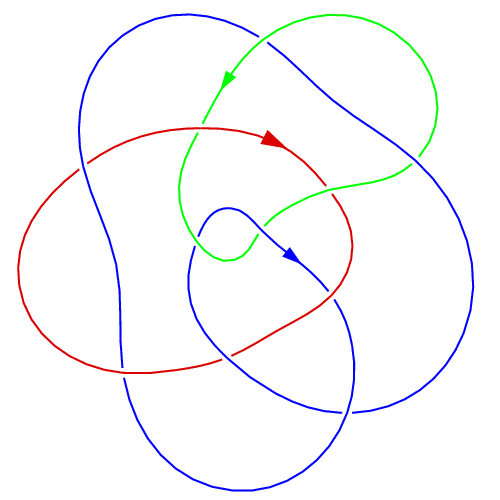
\includegraphics[width=\linewidth]{../data/link_mirror.png} 
            \subcaption{lustro $mL$}
        \end{minipage}
        \begin{minipage}[b]{.32\linewidth}
            \centering 
            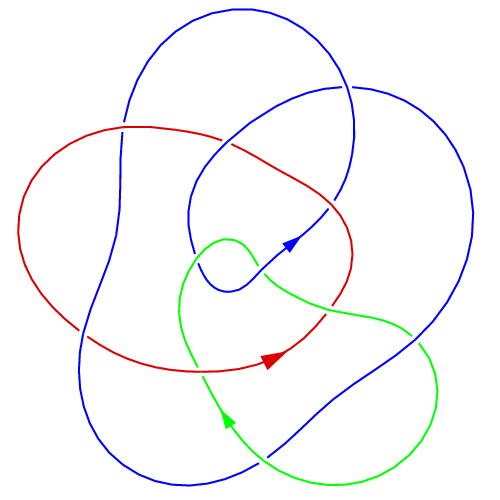
\includegraphics[width=\linewidth]{../data/link.png} 
            \subcaption{przykładowy splot $L$}
        \end{minipage}
        \begin{minipage}[b]{.32\linewidth}
            \centering 
            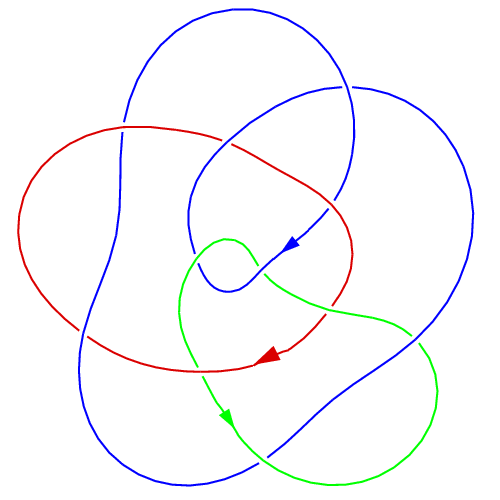
\includegraphics[width=\linewidth]{../data/link_reverse.png} 
            \subcaption{rewers $rL$}
        \end{minipage}
    \end{figure}
\end{definition}

Na lewym obrazku odbiliśmy diagram względem poziomej prostej,
ale równie dobrze można po prostu zamienić każde nadskrzyżowanie na podskrzyżowanie.
Zauważmy, że wykonując powyższe operacje na węźle możemy otrzymać mniej niż czterech różne obiekty
($L$, $mL$, $rL$, $mrL$) -- na przykład trójlistnik jest własnym rewersem, ale nie lustrem.

\begin{definition}
    Istnieje pięć typów symetrii węzłów:
    całkowicie chiralny albo skrętny (węzły $K$, $rK$, $mK$ są parami nierównoważne),
    odwracalny ($K \cong rK$),
    zwierciadlany ujemnie ($K \cong mrK$),
    zwierciadlany dodatnio ($K \cong mK$) oraz
    całkowicie zwierciadlany ($rK \cong K \cong mK$).
\end{definition}

Węzeł $9_{32}$ jest całkowicie skrętny. 
Ósemka jest zwierciadlana, trójlistnik jest odwracalny,
zaś $8_{17}$ to najprostszy przykład węzła nieodwracalnego.
Ten ostatni fakt jest jednak daleki od oczywistego -- 
sześćdziesiąt lat temu nie było pewne,
czy węzły nieodwracalne w ogóle istnieją.
W roku 1962 Ralph Fox wskazał kilku kandydatów do tego tytułu.
Hale Trotter odkrył rok później nieskończoną rodzinę nieodwracalnych precli (patrz \ref{def:pretzel}).
Obecnie wiadomo, że prawie wszystkie węzły są nieodwracalne (\cite[s.~46]{murasugi96}).
Wszystkie węzły torusowe są skrętne.

\begin{proposition}[Trotter, 1963] \label{trotter}
    Precel $(p, q, r)$, gdzie $p, q, r$ sa parami różnymi liczbami całkowitymi, nie jest odwracalny.
\end{proposition}

\begin{proof}
    Praca \cite{trotter63} sprowadza w elementarny sposób problem do pytania, czy pewna grupa posiada inwersję.
\end{proof}

Tait odnosił wrażenie, że zwierciadlane węzły mają parzysty indeks skrzyżowań,
ale Hoste (Thistlethwaite?) znalazł w 1998 kontrprzykład o piętnastu skrzyżowaniach.
Jest on jedynym znanym nam dzisiaj.
Hipoteza Taita jest prawdziwa dla węzłów pierwszych, alternujących.

Poniższa tabela oparta jest (kolejno) o ciągi 
\href{https://oeis.org/A051766}{51766}, 
\href{https://oeis.org/A051769}{51769}, 
\href{https://oeis.org/A051768}{51768}, 
\href{https://oeis.org/A051767}{51767}, 
\href{https://oeis.org/A052400}{52400}, 
z bazy danych ``The On-Line Encyclopedia of Integer Sequences'' (OEIS).

\begin{table}[h]
    \centering
    \begin{tabular}{@{}*{20}l@{}} \toprule
        skrzyżowania & 3 & 4 & 5 & 6 & 7 & 8 & 9 & 10 & 11 & 12 & 13 & 14 \\ \midrule
        całkowicie skrętne & 0 & 0 & 0 & 0 & 0 & 0 & 2 & 27 & 187 & 1103 & 6919 & 37885 \\
        odwracalne & 1 & 0 & 2 & 2 & 7 & 16 & 47 & 125 & 365 & 1015 & 3069 & 8813 \\
        $-$ zwierciadlane & 0 & 0 & 0 & 0 & 0 & 1 & 0 & 6 & 0 & 40 & 0 & 227 \\
        $+$ zwierciadlane & 0 & 0 & 0 & 0 & 0 & 0 & 0 & 0 & 0 & 1 & 0 & 6 \\
        zwierciadlane & 0 & 1 & 0 & 1 & 0 & 4 & 0 & 7 & 0 & 17 & 0 & 41 \\
        \bottomrule
        \hline
    \end{tabular}
    \caption{Liczba węzłów o poszczególnych typach symetrii}
    \label{tablica_wezlow}
\end{table}

% Koniec podsekcji Operacje na pojedynczym splocie

\subsection{Sumy wielu węzłów} % (fold)
\label{sub:knot_sum}
Suma spójna węzłów to szczególny przypadek sklejenia dwóch rozmaitości wzdłuż brzegu.

\begin{definition}
    Niech $L_1, L_2$ będą splotami.
    Ich \textbf{sumą niespójną}, $L_1 \sqcup L_2$,
    jest teoriomnogościowa suma rozłączna splotów
    $L_1$ i $L_2$ leżących po różnych stronach pewnej płaszczyzny.
\end{definition}

\begin{definition}
    Nacinając dwa zorientowane węzły w dwóch bliskich punktach i 
    ponownie zszywając je dwoma łukami nieprzecinającymi już
    istniejących otrzymujemy \textbf{sumę spójną}, $K_1 \shrap K_2$.
    \[
        \begin{tikzpicture}[baseline=-0.65ex,scale=0.1]
        \begin{knot}[clip width=5, flip crossing/.list={5}, ignore endpoint intersections=false,]
            \strand[thick] (-3.5, -3.5) [in=down, out=up] to (3.5, 3.5);
            \strand[thick] (3.5, 3.5) [in=right, out=up] to (-4.5, 10);
            \strand[thick] (-4.5, 10) [in=up, out=left] to (-10, 3.5);
            \strand[thick] (-10, 3.5) to (-10, -3.5);
            \strand[thick] (-10, -3.5) [in=left, out=down] to (-4.5, -10);
            \strand[thick] (-4.5, -10) [in=down, out=right] to (3.5, -3.5);
            \strand[thick] (3.5, -3.5) [in=down, out=up] to (-3.5, 3.5);
            \strand[thick] (-3.5, 3.5) [in=left, out=up] to (4.5, 10);
            \strand[thick] (4.5, 10) [in=up, out=right] to (10, 3.5);
            \strand[thick, -Latex] (10, 3.5) to (10, -3.5);
            \strand[thick] (10, -3.5) [in=right, out=down] to (4.5, -10);
            \strand[thick] (4.5, -10) [in=down, out=left] to (-3.5, -3.5);
            \node at (0, -15) {$K_1$};
        \end{knot}
        \end{tikzpicture}
        \shrap
        \begin{tikzpicture}[baseline=-0.65ex,scale=0.1]
        \begin{knot}[clip width=5, flip crossing/.list={6}, ignore endpoint intersections=false,]
            \strand[thick] (-3.5, -3.5) [in=down, out=up] to (3.5, 3.5);
            %\strand[thick] (3.5, 3.5) [in=right, out=up] to (-4.5, 10);
            %\strand[thick] (-4.5, 10) [in=up, out=left] to (-10, 3.5);
            \strand[thick] (-10, -3.5) [in=left, out=up] to (0, 6.5);
            \strand[thick, Latex-] (-10, -3.5) [in=left, out=down] to (-4.5, -10);
            \strand[thick] (-4.5, -10) [in=down, out=right] to (3.5, -3.5);
            \strand[thick] (3.5, -3.5) [in=down, out=up] to (-3.5, 3.5);
            %\strand[thick] (-3.5, 3.5) [in=left, out=up] to (4.5, 10);
            %\strand[thick] (4.5, 10) [in=up, out=right] to (10, 3.5);
            \strand[thick] (10, -3.5) [in=right, out=up] to (0, 6.5);
            \strand[thick] (10, -3.5) [in=right, out=down] to (4.5, -10);
            \strand[thick] (4.5, -10) [in=down, out=left] to (-3.5, -3.5);
            %
            \strand[thick] (-3.5, 3.5) [in=left, out=up] to (0, 10);
            \strand[thick] (3.5, 3.5) [in=right, out=up] to (0, 10);
            \node at (0, -15) {$K_2$};
        \end{knot}
        \end{tikzpicture}
        =
        \begin{tikzpicture}[baseline=-0.65ex,scale=0.1]
        \begin{knot}[clip width=5, flip crossing/.list={5, 22, 23}, ignore endpoint intersections=false,]
            \strand[thick] (-18.5, -3.5) [in=down, out=up] to (-11.5, 3.5);
            \strand[thick] (-11.5, 3.5) [in=right, out=up] to (-19.5, 10);
            \strand[thick] (-19.5, 10) [in=up, out=left] to (-25, 3.5);
            \strand[thick] (-25, 3.5) to (-25, -3.5);
            \strand[thick] (-25, -3.5) [in=left, out=down] to (-19.5, -10);
            \strand[thick] (-19.5, -10) [in=down, out=right] to (-11.5, -3.5);
            \strand[thick] (-11.5, -3.5) [in=down, out=up] to (-18.5, 3.5);
            \strand[thick] (-18.5, 3.5) [in=left, out=up] to (-10.5, 10);
            \strand[thick] (-10.5, 10) [in=left, out=right] to (-5, 2);
            \strand[thick, -Latex] (-5, 2) to (-5+6, 2);
            \strand[thick] (5, 2) to (-5+6, 2);
            \strand[thick] (3, -2) to [in=left, out=right] (10.5, -10);
            \strand[thick, -Latex] (3, -2) to (0, -2);
            \strand[thick] (-5, -2) to (0, -2);
            \strand[thick] (-5, -2) [in=right, out=left] to (-10.5, -10);
            \strand[thick] (-10.5, -10) [in=down, out=left] to (-18.5, -3.5);
            %%%
            \strand[thick] (11.5, -3.5) [in=down, out=up] to (18.5, 3.5);
            \strand[thick] (-10 +15, 2) [in=left, out=right] to (15, 6.5);
            \strand[thick] (10.5, -10) [in=down, out=right] to (18.5, -3.5);
            \strand[thick] (18.5, -3.5) [in=down, out=up] to (11.5, 3.5);
            \strand[thick] (25, -3.5) [in=right, out=up] to (15, 6.5);
            \strand[thick] (25, -3.5) [in=right, out=down] to (19.5, -10);
            \strand[thick] (19.5, -10) [in=down, out=left] to (11.5, -3.5);
            \strand[thick] (11.5, 3.5) [in=left, out=up] to (15, 10);
            \strand[thick] (18.5, 3.5) [in=right, out=up] to (15, 10);
            %%%
            \node at (0, -15) {$K_1 \shrap K_2$};
        \end{knot}
        \end{tikzpicture}
        \]
\end{definition}

Uogólnieniem tego działania oraz 
(nieopisanej w naszej pracy) operacji \emph{plumbing}
jest suma Murasugiego, dobrze wyjaśniona w czwartym rozdziale \cite{kawauchi96}.

Ważna jest orientacja składników:
suma dwóch trójlistników może być,
w zależności od ich orientacji,
węzłem babskim\todo{nazewnictwo pochodzi od żeglarzy, nie matematyków} lub prostym.
Fox pokazał w 1952 roku,
że dopełnienia tych dwóch węzłów nie są homeomorficzne.
Suma przeciwnie skręconych trójlistników jest plastrowa
(definicja \ref{def:slice_knot}),
natomiast tak samo skręconych -- nie.

\begin{proposition}
    Suma spójna jest dobrze określonym działaniem.
\end{proposition}

Suma spójna nie jest dobrze określona dla splotów:
nie istnieje kanoniczny wybór, które składowe łączyć ze sobą.

\begin{proof}
    Niech dane będą węzły $K_1$ oraz $K_2$
    oraz dwa różne łuki $\gamma_1$, $\gamma_2$,
    których można użyć do konstrukcji sumy spójnej.
    Skurczmy $K_1$, przeciągnijmy najpierw przez łuk $\gamma_1$, a następnie wzdłuż węzła $K_2$.
    Teraz wystarczy odwrócić ten proces z $\gamma_2$ w miejscu $\gamma_1$.
\end{proof}

\begin{proposition}
    Suma spójna zorientowanych węzłów posiada następujące własności:
    \begin{enumerate}[leftmargin=*]
    \itemsep0em
        \item jest łączna:
        $(K_1 \shrap K_2) \shrap K_3 \simeq K_1 \shrap (K_2 \shrap K_3)$,
        \item jest przemienna:
        $K_1 \shrap K_2 \simeq K_2 \shrap K_1$,
        \item posiada element neutralny:
        $K_1 \shrap \MalyNieWezel \simeq \MalyNieWezel \shrap K_1 \simeq K_1$.
    \end{enumerate}
\end{proposition}

Prosty dowód tego faktu pozostawiamy Czytelnikowi.
Pokażemy za to, iż węzły z sumą spójną nie tworzą grupy -- brakuje elementów przeciwnych.

\begin{proposition}
    Jeśli $K \shrap L = \NieWezel$, to $K = L = \NieWezel$.
\end{proposition}

\begin{proof}[Niedowód]
    Technika ta zwana jest szwindlem Mazura.
    Załóżmy, że $K \shrap L = \NieWezel$ i dopuśćmy wyjątkowo węzły dzikie.
    Skonstruujmy sumę $K \shrap L \shrap K \shrap \ldots$,
    przy czym kolejne składniki powinny zmniejszać się,
    aby ich suma nadal była węzłem.
    Wtedy
    \begin{align*}
        K & \simeq K \shrap [(L \shrap K) \shrap (L \shrap K) \ldots] \\
         & \simeq (K \shrap L) \shrap (K \shrap L) \shrap \ldots
         \simeq \NieWezel \shrap \NieWezel \shrap \ldots
         \simeq \NieWezel.
    \end{align*}
    Analogicznie pokazujemy, że $L \simeq \NieWezel$.
\end{proof}

Później poznamy prawdziwy, oparty na topologii algebraicznej, dowód.
Połączymy fakty \ref{genus_one} oraz \ref{genus_sum}.

Półgrupę węzłów z operacją sumy spójnej można ulepszyć do grupy na dwa sposoby:
albo poprzez zmianę działania, w jakie jest wyposażona,
albo osłabiając definicję węzłów równoważnych.
Drugi pomysł jest dużo lepszy niż pierwszy.
Na początku lat pięćdziesiątych J. Millnor wprowadził do matematyki pojęcie zgodności
(z angielskiego \emph{concordance}), które zastąpiło zwykłą równoważność.
Element neutralny nowej grupy to węzły plastrowe, ich opis leży w sekcji \ref{sec:slice}.
Zagadnienia te zakorzenione są w czterowymiarowej topologii.

% Koniec podsekcji Sumy wielu węzłów

% Koniec sekcji Operacje na węzłach

\section{Węzły pierwsze}
\label{sec:prime_knots}
Istnieje węzłowy odpowiednik liczb pierwszych.
Jest on ściśle związany z~podaną wyżej operacją sumy spójnej.
Do jego dostatecznie dobrego zrozumienia wymagana jest znajomość powierzchni Seiferta (opisanych w~sekcji \ref{sec:genus}).

\begin{definition}
    \label{primeknot}
    \index{węzeł!pierwszy}
    Nietrywialny węzeł nazywamy \textbf{pierwszym},
    kiedy nie można przedstawić go jako sumy spójnej $K_1 \shrap K_2$
    dwóch nietrywialnych węzłów $K_1, K_2$ (nie jest złożony).
\end{definition}

Okazuje się, że jeśli alternujący splot nie jest pierwszy,
to każdy jego alternujący diagram jest złożony.
Jako pierwszy fakt ten został wykazany przez Menasco w~\cite{menasco84}.
Dowód opiera się na multiplikatywności wielomianu BLM/Ho (opisuje go definicja \ref{def:blm_ho}).

Czy węzłów pierwszych jest nieskończenie wiele?
Tak (patrz fakt \ref{infty_primes}), potrafimy nawet oszacować liczbę $K_n$ węzłów pierwszych oraz $L_n$ splotów pierwszych.
W roku 1987 C. Ernst, D. Sumners w~oparciu o~wyniki Thistlethwaite'a, Kauffmana, oraz Murasugiego dotyczące węzłów alternujących pokazali w~\cite{ernst87}, że $K_n \ge \frac 1 3 (2^{n- 2} - 1)$, przy czym węzły lustrzane traktowane są jako różne.
Dokładniej:

\begin{proposition}
    Niech $f(n)$ oznacza liczbę węzłów dwumostowych o indeksie skrzyżowaniowym $n$.
    Wtedy
    \begin{equation}
        f(n) = \begin{cases}
        \frac 13 (2^{n-2} - 1) & \text{dla } n = 2k \ge 4 \\
        \frac 13 (2^{n-2} + 2^{(n-1)/2}) & \text{dla } n = 4k + 1 \ge 5 \\
        \frac 13 (2^{n-2} + 2^{(n-1)/2} + 2) & \text{dla } n = 4k + 3 \ge 7
        \end{cases}
    \end{equation}
\end{proposition}


Welsh rozpatruje w \cite{welsh92} węzły bez orientacji i znajduje poniższe ograniczenia.
Nie wiadomo, czy zwykłe granice istnieją.
\begin{equation}
    2.68 \le \liminf_{n \to \infty}  \sqrt[n]{K_n} \le \limsup_{n \to \infty} \sqrt[n]{L_n} \le \frac {27}{2}.
\end{equation}

% "On the number of knots and links" (MR1218230)

Czy niewęzeł nie daje się zapisać jako suma dwóch innych węzłów?
Byłoby to skrajnie niepożądane, gdyż każdy węzeł jest naturalnie spójną sumą siebie oraz niewęzła.
Na szczęście przy pomocy powierzchni Seiferta można pokazać, że tak się nie dzieje (jest to wniosek \ref{no_inverses}).
Prawdziwe jest dużo mocniejsze stwierdzenie,
którego nie udowodnimy ze względu na niedostatecznie rozwinięty aparat matematyczny.
Należy o~nim myśleć jak o~analogonie zasadniczego twierdzenia arytmetyki.

\begin{theorem}[Schubert, 1949]
    \label{thm:schubert}
    Każdy różny od niewęzła węzeł rozkłada się jednoznacznie na węzły pierwsze
    (jeśli tylko pominąć kolejność składników).
\end{theorem}

Schubert podał geometryczny dowód oparty o powierzchnie Seiferta; wyraził go w języku PL-rozmaitości (\cite{schubert49}), ale niedużym wysiłkiem można dokonać adaptacji do gładkiego świata.
Praca Schuberta korzysta z twierdzenia Alexandera, że 2-sfera w przestrzeni $\R^3$ ogranicza dysk, i jego odpowiednika dla torusów w $S^3$

My pokażemy tylko, że rozkład istnieje i jest skończony, to fakt \ref{genus_sum}.
% koniec sekcji Węzły pierwsze

\section{Niezmienniki liczbowe}
Jak wspomnieliśmy na początku rozdziału, sprawdzenie,
czy dwa diagramy przedstawiają sploty równoważne,
jest uciążliwym i~czasochłonnym zadaniem.
Aby je uprościć, podamy opis kilku prostych niezmienników o~całkowitych wartościach.
Zachodzą implikacje:
sploty równoważne $\Rightarrow$ ta sama wartość niezmiennika
oraz różne wartości niezmiennika $\Rightarrow$ różne sploty.

\subsection{Indeks skrzyżowaniowy} % (fold)
\label{sub:crossing_number}
\index{indeks!skrzyżowaniowy}
Z angielskiego \emph{crossing number}.

\begin{definition}
    Indeks skrzyżowaniowy $\operatorname{cr}(L)$ splotu $L$ to
    minimalna liczba skrzyżowań widocznych na diagramie,
    który przedstawia splot $L$.
\end{definition}

Jeśli $K_1, K_2$ są alternującymi węzłami o~$c_1, c_2$ skrzyżowaniach, to istnieje alternujący diagram ich sumy $K_1 \shrap K_2$ o~$c_1 + c_2$ skrzyżowaniach.
Lackenby w~pracy \cite{lackenby09} pokazał, że dla pewnej stałej $N \le 152$ zachodzi
\[
    \frac 1 N \sum_{i=1}^n \operatorname{cr} K_i \le \operatorname{cr} \left(\bigshrap_{i=1}^n K_i\right) \le \sum_{i=1}^n \operatorname{cr} K_i.
\]
(Tylko pierwsza nierówność jest ciekawa).
Jego argumentu (wykorzystującego powierzchnie normalne) nie można poprawić tak, by otrzymać stałą $N = 1$.
Wiadomo jednak, że indeks skrzyżowaniowy jest addytywny dla niektórych klas węzłów: alternujących (\cite{kauffman88}), adekwatnych\footnote{Węzły adekwatne nie pojawiają się na żadnej innej stronie tej książki.} czy torusowych (\cite{gruber03}).

\begin{theorem}[Bankwitz, 1930] \label{thm:bankwitz}
    Wyznacznik węzła alternującego jest nie mniejszy od jego indeksu skrzyżowaniowego.
\end{theorem}

\begin{proof}
    Pierwszy dowód podał Bankwitz w~pracy \cite{bankwitz30}.
    Inne rozumowanie przedstawił Crowell w~(łatwo dostępnym) artykule o~niespodziewanym tytule Nonalternating links z~1957 r.
\end{proof}

% Koniec podsekcji Indeks skrzyżowaniowy

\subsection{Liczba gordyjska} % (fold)
\label{sub:unknotting_number}
\index{liczba!gordyjska}
Z angielskiego \emph{unknotting number}.

\begin{definition}
    Liczba gordyjska $\operatorname{u}(K)$ węzła $K$ to minimalna liczba skrzyżowań,
    które trzeba odwrócić na pewnym jego diagramie, by dostać niewęzeł.
    Liczba $u$ nie musi być osiągana przez diagram o~minimalnej liczbie skrzyżowań.
\end{definition}

Dotychczas wyznaczono liczbę gordyjską dla prawie wszystkich węzłów pierwszych o~co najwyżej dziesięciu skrzyżowaniach,
Cha i~Livingston podają następującą listę wyjątków:
$10_{11}$, $10_{47}$, $10_{51}$, $10_{54}$, $10_{61}$, $10_{76}$, $10_{77}$, $10_{79}$, $10_{100}$ (stan na rok 2008).
S. Bleiler odkrył w~\cite{bleiler84} fascynujący przykład wymiernego węzła $2$-gordyjskiego,
czego świadkiem nie może być diagram o~minimalnej liczbie skrzyżowań
(ponieważ, co jeszcze bardziej fascynujące, węzeł ten posiada tylko jeden diagram o~dziesięciu skrzyżowaniach z~trzema do odwrócenia).
Koduje go liczba $29/6$, w~tabeli węzłów figuruje jako $10_8$.
Stojmenow w~\cite{stoimenow01} pokazuje, że jeden węzeł może mieć kilka diagramów minimalnych,
z których tylko niektóre są świadkiem $1$-gordyjskości (są to między innymi $14_{36750}$ oraz $14_{36760}$.)

Coward, Lackenby dowiedli w~\cite{coward11}, że jeśli $K$ jest 1-gordyjski i~o genusie 1, to z~dokładnością do pewnej relacji równoważności, tylko jedna zmiana skrzyżowania rozwiązuje go; chyba że $K$ jest ósemką -- wtedy takie zmiany są dwie.
Kanenobu, Murakami oraz Kohn dwadzieścia lat wcześniej wiedzieli, że wymierne sploty 1-gordyjskie posiadają rozwiązujące skrzyżowanie na minimalnym diagramie (\cite{kanenobu86}, \cite{kohn91}).

Jeśli odwrócenie pewnych skrzyżowań daje niewęzeł, to odwrócenie pozostałych także.
To daje proste, choć niezbyt pomocne oszacowanie liczby gordyjskiej: $2 \operatorname{u} (K) \le \operatorname{cr} (K)$.
Borodzik oraz Friedl podali niedawno całkiem mocne ograniczenia na liczbę gordyjską w~pracach \cite{borodzik14} i~\cite{borodzik15} opierając się o~parowanie Blanchfielda
(poprawiając ograniczenia z~sygnatury Levine'a-Tristrama, indeksu Nakanishiego oraz przeszkodą Lickorisha).
Dwadzieścia pięć węzłów o~co najwyżej dwunastu skrzyżowaniach ma liczbę gordyjską równą co najmniej trzy, co trudno pokazać innymi metodami.

Dla każdego nietrywialnego splotu istnieje diagram wymagający odwrócenia dowolnie wielu skrzyżowań (dowód zawiera praca \cite{taniyama09} Taniyamy).
Pokazany jest tam jeszcze jeden godny uwagi fakt.
Jeśli liczba gordyjska diagramu $D$ wynosi $\frac 12 (c(D) - 1)$,
co jest maksymalną możliwą wartością zgodnie z~naszym prostym ograniczeniem,
to węzeł jest $(2,p)$-torusowy albo wygląda jak diagram niewęzła po pierwszym ruchu Reidemeistera.

% Liczba gordyjska nietrywialnego węzła skręconego (definicja \ref{twist_knots}) to jeden, wystarczy bowiem rozwiązać jego splecione końce.
Patrz także stwierdzenie \ref{torus_unknotting}.

Suma dwóch węzłów $1$-gordyjskch jest $2$-gordyjska, pokazał to Scharleman.
Od początku teorii węzłów podejrzewano dużo więcej:

\begin{conjecture}
    Niech $K, J$ będą węzłami.
    Wtedy $u(K \shrap J) = u(K) + u(J)$, czyli liczba gordyjska jest addytywna.
\end{conjecture}

Z tej nieudowodnionej do dzisiaj (stan na 2018) hipotezy można wyciągnąć wniosek,
że jeśli do rozwiązania węzła wystarcza odwrócenie skrzyżowania, to jest pierwszy.
Podejrzewał to H. Wendt w~1937 roku,
kiedy policzył liczbę gordyjską węzła babskiego używając homologii rozgałęzionego nakrycia cyklicznego.

\begin{proposition}
    Węzły $1$-gordyjskie są pierwsze.
\end{proposition}

\begin{proof}[Niedowód]
    W pracy \cite{scharleman85} z~1985 roku M. Scharleman podał dość zawiłe uzasadnienie, w~które zamieszane były grafy planarne.
\end{proof}

W pracy \cite{shimizu14} Ayaka Shimizu pokazuje przykład innej operacji rozwiązującej węzły, ale nie wszystkie sploty:
zmianę skrzyżowań wokół obszaru na diagramie.

Liczbę gordyjską można uogólnić w naturalny sposób do metryki.
Mianowicie mając dane dwa węzły $K_0, K_1$, rozpatrzmy wszystkie homotopie $f : [0,1] \times S^1 \to \R^3$ takie, że wszystkie funkcje $f_t$ są zanurzeniami z co najwyżej jednym punktem podwójnym.
Zażądajmy dodatkowo, by styczne do krótkich łuków, które przecinają się w tym punkcie, były od siebie różne.
Odległością gordyjską między węzłami $K_0, K_1$ jest minimalna liczba podwójnych punktów, jakie posiada homotopia $f$.

Przestrzeń węzłów z~tą metryką bywa sprzeczna z~intuicją: twierdzenie C~z~pracy \cite{gambaudo05} głosi, że zawiera ona prawie idealną kopię przestrzeni euklidesowej dowolnego wymiaru.
Dokładniej:

\begin{proposition}
    Dla każdej liczby całkowitej $d \ge 1$ istnieje funkcja $\xi: \Z^d \to \mathcal{K}$, dodatnie stałe $A, B, C$ oraz norma $\|\cdot\|$ na przestrzeni $\R^d$ takie, że spełniona jest podwójna nierówność
    \[
        A\|x-y\|  - B \le d(\xi(x), \xi(y)) \le C\|x-y\|.
    \]
\end{proposition}

Dowód korzysta z grup warkoczowych, które poznamy w sekcji \ref{sec:braid}.

\begin{conjecture}[Bernhard 1994, Jablan 1998] \label{bernhard_jablan}
    Każdy węzeł $K$ posiada diagram $D$ realizujący liczbę gordyjską oraz skrzyżowanie, którego odwrócenie daje nowy węzeł $K'$ z diagramem $D'$ o mniejszej liczbie gordyjskiej: $u(D') < u(D)$.
\end{conjecture}

Gdyby hipoteza była prawdziwa, mielibyśmy dość prosty algorytm do wyznaczania liczby gordyjskiej $u(K)$: wystarczy skonstruować skończenie wiele diagramów minimalnych dla węzła $K$, odwracać kolejne skrzyżowania i szukać rekursywnie liczb gordyjskich nowych węzłów.
Hipoteza jest prawdziwa dla węzłów do jedenastu skrzyżowań (patrz baza danych KnotInfo C. Livingstona) i splotów o dwóch składowych do dziewięciu skrzyżowań, pokazał to Kohn w pracy \cite{kohn93} z 1993 (!) roku.
Brittenham, Hermiller twierdzą, że hipoteza jest fałszywa.

% Koniec podsekcji Liczba gordyjska

\subsection{Liczba mostowa} % (fold)
\label{sub:bridge_index}
\index{liczba!mostowa}
Z angielskiego \emph{bridge number}.
Wprowadzona w~1954 przez Schuberta.
\begin{definition}
    Liczba mostowa $\operatorname{br}(K)$ to minimalna liczba mostów:
    długich łuków, które biegną przez nadskrzyżowania.
\end{definition}

Można pokazać, że $n$-mostowe węzły rozkładają się na sumę dwóch trywialnych $n$-supłów.

\begin{proposition}
    Niech $K_1, K_2$ będą węzłami.
    Wtedy $\operatorname{br} (K_1) + \operatorname{br}(K_2) = \operatorname{br}(K_1 \# K_2) + 1$.
\end{proposition}

\begin{proof}[Nieedowód]
    Schubert pokazał to blisko pół wieku temu w~\cite{schubert54}.
    Nowszy dowód pochodzi od Schultensa, w~artykule \cite{schultens03} skorzystał z~foliacji na brzegu węzła towarzyszącego sateltarnemu.
    Dokładniejszy opis powyższych prac wykraczałby poza zakres tego opracowania, zostanie więc pominięty.
\end{proof}

Tylko jeden węzeł jest jednomostowy, to niewęzeł.
Kolejne w~hierarchii skomplikowania, czyli dwumostowe,
to domknięcia wymiernych supłów, patrz fakt \ref{prp:two_bridge_tangle}.
Węzły trójmostowe pozostają nie do końca zbadane.

\begin{conjecture}
    Jeśli $K$ jest węzłem, to $c(K) \ge 3 br(K) - 3$, przy czym równość zachodzi dokładnie dla niewęzła, trójlistnika i~sumy spójnej trójlistników (rozdział 4.3 z~podręcznika \cite{murasugi96}).
\end{conjecture}

Nie istnieje związek między liczbą mostową oraz gordyjską.
Po pierwsze, węzły torusowe $T_{2,n}$ są dwumostowe, a~ich liczba gordyjska jest duża.
Po drugie, podwojenie węzła (poza specjalnymi przypadkami, jak pokazał Schubert) zwiększa liczbę mostową dwukrotnie; liczba gordyjska takiego podwojenia wynosi $1$.
Podobnie nie ma zależności między liczbą mostową oraz genusem.

% Koniec podsekcji Liczba mostowa

\subsection{Liczba warkoczowa} % (fold)
\label{sub:braid_number}
\index{liczba!warkoczowa}
Z angielskiego \emph{braid number}.
Do jej określenia potrzebna jest definicja \ref{braid_def}.

\begin{definition}
    Liczba warkoczowa to minimalna liczba pasm, na których można zbudować warkocz, którego domknięciem jest wyjściowy węzeł.
\end{definition}

\begin{proposition}
    Węzeł o~$n$ skrzyżowaniach można zapleść na $n - 1$ pasmach.
\end{proposition}

Indeks warkoczowy zależy od orientacji ogniw i~trudno się go wyznacza w~ogólnym przypadku.
Poniższy dowód zakłada znajomość warkoczy (rozdział piąty).

\begin{proposition}
    Indeksem warkoczowym węzła torusowego $K(q, r)$, $rq \neq 0$, jest $\min\{|q|, |r|\}$.
\end{proposition}

\begin{proof}
    Niech $K$ będzie węzłem torusowym typu $(q,r)$ z~minimalnym przedstawieniem jako warkocz $\beta$.
    Z konstrukcji domknięcia (czyli dołączenia rozłącznych półokręgów) wynika,
    że diagram $K$ ma dokładnie $b(K)$ lokalnych maksimów.
    Definicja indeksu mostowego orzeka, iż $br(K) \le b(K)$.
    Bez straty ogólności niech $q > r > 0$.
    Skoro węzeł $K$ powstaje z~$r$-warkocza $(\sigma_{r-1} \ldots \sigma_2\sigma_1)^q$,
    indeks $b(K)$ nie przekracza $r = br(K)$.

    Skorzystaliśmy z~faktu \ref{torus_bridge}.
\end{proof}

% Koniec podsekcji Liczba warkoczowa

\subsection{Indeks zaczepienia} % (fold)
\label{sub:linking_number}
\begin{definition} \label{sign_def}
    Na diagramie zorientowanego splotu, każdemu skrzyżowaniu przypisujemy \textbf{znak} równy $\pm 1$.
    Skrzyżowania dodatnie nazywamy praworęcznymi, ujemne zaś: leworęcznymi.
    \[
        \sign \Bigl(\,\,\begin{tikzpicture}[baseline=-0.65ex,scale=0.07]
        \begin{knot}[clip width=5]
        \strand[semithick,-Latex] (-5,-5) -- (5,5);
        \strand[semithick,Latex-] (-5,5) -- (5,-5);
        \end{knot}\end{tikzpicture}\,\,\Bigr) = +1 \quad
        \sign \Bigl(\,\,\begin{tikzpicture}[baseline=-0.65ex,scale=0.07]
        \begin{knot}[clip width=5, flip crossing/.list={1}]
        \strand[semithick,-Latex] (-5,-5) -- (5,5);
        \strand[semithick,Latex-] (-5,5) -- (5,-5);
        \end{knot}\end{tikzpicture}\,\,\Bigr) = -1
    \]
\end{definition}

\begin{definition} \label{sign_def}
    \index{indeks!zaczepienia}
    Niech $L = K_1 \sqcup K_2$ będzie splotem o dwóch ogniwach.
    Wielkość
    \[
        \operatorname{lk}(K_1, K_2) = \frac 12 \sum_i \sign c_i,
    \]
    gdzie sumowanie rozciąga się na wszystkie skrzyżowania, gdzie spotykają się łuki z różnych ogniw, nazywamy \textbf{indeksem zaczepienia} węzłów $K_1, K_2$.
    Ogólniej, jeśli $L = K_1 \sqcup \ldots \sqcup K_n$ jest splotem o $n$ ogniwach, to jego indeks zaczepienia wyznacza wzór $\operatorname{lk}(L) = \sum_{i < j} \operatorname{lk}(K_i, K_j)$.
\end{definition}

Zauważmy, że indeks zaczepienia splotu Hopfa wynosi $1$, natomiast splotu Whiteheada $0$.
Są zatem istotnie różne.
W obydwu przypadkach indeks zaczepienia jest liczbą całkowitą, nie stanowi to przypadku.
Na mocy twierdzenia Jordana $\operatorname{lk}$ jest funkcją o całkowitych wartościach.

\begin{proposition}
    Indeks zaczepienia jest dobrze określonym niezmiennikiem zorientowanych splotów.
\end{proposition}

\begin{proof}
    Sprawdźmy wpływ ruchów Reidemeistera na wartość
    $\operatorname{lk}(L)$:

    \[
        \fbox{
        \begin{tikzpicture}[baseline=-0.65ex,scale=0.07]
        \begin{knot}[clip width=5]
        \strand[semithick] (-10,10) .. controls (-10,2) and (-10,2) .. (-6,-2);
        \strand[semithick] (-10,-10) .. controls (-10,-2) and (-10,-1) .. (-9,0);
        \strand[semithick] (-7,1) -- (-6,2);
        \strand[semithick] (-6,2) .. controls (2,9) and (2,-9) .. (-6,-2);
        \end{knot}
        \end{tikzpicture}
        $\stackrel{R_1}{\cong} \,\,$
        \begin{tikzpicture}[baseline=-0.65ex,scale=0.07]
        \begin{knot}[clip width=5]
        \strand[semithick] (0,10) -- (0,-10);
        \end{knot}
        \end{tikzpicture}}
        %%%
        \quad \fbox{
        \begin{tikzpicture}[baseline=-0.65ex,scale=0.07]
        \begin{knot}[clip width=5]
        \strand[semithick] (4,-10) .. controls (4,-4) and (-4,-4) .. (-4,0);
        \strand[semithick] (4,10) .. controls (4, 4) and (-4, 4) .. (-4,0);
        \strand[semithick] (-4,-10) .. controls (-4,-4) and (4,-4) .. (4,0);
        \strand[semithick] (-4,10) .. controls (-4, 4) and (4,4) .. (4,0);
        \node[blue] at (-4,4)[left] {$a$};
        \node[blue] at (-4,-4)[left] {$-a$};
        \end{knot}
        \end{tikzpicture}
        $\stackrel{R_2}{\cong} \,\,$
        \begin{tikzpicture}[baseline=-0.65ex,scale=0.07]
        \begin{knot}[clip width=5]
        \strand[semithick] (4,-10) .. controls (4,-4) and (1,-4) .. (1,0);
        \strand[semithick] (4,10) .. controls (4, 4) and (1, 4) .. (1,0);
        \strand[semithick] (-4,-10) .. controls (-4,-4) and (-1,-4) .. (-1,0);
        \strand[semithick] (-4,10) .. controls (-4, 4) and (-1,4) .. (-1,0);
        \end{knot}
        \end{tikzpicture}}
        %%%
        \quad \fbox{
        \begin{tikzpicture}[baseline=-0.65ex,scale=0.07]
        \begin{knot}[clip width=5, flip crossing/.list={1,2,3}]
        \strand[semithick] (-10,-10) -- (10,10);
        \strand[semithick] (-10,10) -- (10,-10);
        \strand[semithick] (-10,-2) .. controls (-4, -2) and (-4,8) .. (0,8);
        \strand[semithick] (10,-2) .. controls (4, -2) and (4,8) .. (0,8);
        \node[blue] at (-6,4)[left] {$a$};
        \node[blue] at (6,4)[right] {$b$};
        \node[blue] at (0,-2)[below] {$c$};
        \end{knot}
        \end{tikzpicture}
        $\stackrel{R_3}{\cong} \,\,$
        \begin{tikzpicture}[baseline=-0.65ex,scale=0.07]
        \begin{knot}[clip width=5, flip crossing/.list={1,2,3}]
        \strand[semithick] (-10,-10) -- (10,10);
        \strand[semithick] (-10,10) -- (10,-10);
        \strand[semithick] (-10,2) .. controls (-4, 2) and (-4,-8) .. (0,-8);
        \strand[semithick] (10,2) .. controls (4, 2) and (4,-8) .. (0,-8);
        \node[blue] at (-6,-4)[left] {$a$};
        \node[blue] at (6,-4)[right] {$b$};
        \node[blue] at (0,2)[above] {$c$};
        \end{knot}
        \end{tikzpicture}}
    \]
    Na mocy twierdzenia Reidemeistera dowód został zakończony.
\end{proof}

Kawauchi definiuje jeszcze \emph{twisting number}: sumę spinów po wszystkich składowych.

% Koniec podsekcji Indeks zaczepienia

\subsection{Sygnatura} % (fold)
\label{sub:signature}
\index{sygnatura}
Sygnatura pojawia się w~fakcie \ref{slice_signature}.

\begin{definition}
    Sygnatura to niezmiennik topologiczny zadany (kłębiastą) relacją rekurencyjną:
    \begin{itemize}[leftmargin=*]
    \itemsep0em
        \item $\sigma (\LittleUnknot) = 0$,
        \item $\sigma (K_+) - \sigma (K_-) \in \{0, 2\}$,
        \item $4 \mid \sigma (K)$ wtedy i~tylko wtedy, gdy $\nabla(2i) > 0$ (wielomian Conwaya).
    \end{itemize}
\end{definition}

\begin{proposition} \label{prop_sigma_inverse}
    Mamy $\sigma(K^*) = -\sigma(K)$ oraz $\sigma(-K) = \sigma(K)$.
\end{proposition}

\begin{proof}
    To jest twierdzenie 6.4.5 z podręcznika \cite{murasugi96}.
\end{proof}

\begin{proposition} \label{prop_sigma_additive}
    Sygnatura jest addytywna: $\sigma(K_1 \shrap \ldots \shrap K_n) = \sum_{k=1}^n \sigma(K_k)$.
\end{proposition}

Węzły achiralne mają zerową sygnaturę, zatem trójlistnik nie jest achiralny.
Z faktów \ref{prop_sigma_inverse} oraz \ref{prop_sigma_additive} wynika, że suma tak samo skręconych trójlistników nie jest achiralna ($\sigma = \pm 4$), natomiast węzeł prosty (suma różnie skręconych) ma zerową sygnaturę i jak można przekonać się ze standardowego diagramu, jest achiralny.

Sygnatura pozwala uzyskać proste oszacowanie liczby gordyjskiej od dołu:

\begin{proposition}
    Mamy $2 u(K) \ge |\sigma(K)|$.
\end{proposition}

\begin{proof}
    To jest twierdzenie 6.4.8 z podręcznika \cite{murasugi96}.
\end{proof}

Nie istnieje bezpośredni związek między sygnaturą i~liczbą mostową.
Węzeł torusowy $T_{2,n}$ jest dwumostowy, jego sygnatura wynosi $n - 1$.
Suma spójna węzłów prostych ma zerową sygnaturę i~nieograniczoną liczbę mostową.
Wynika to z~ogólniejszego faktu:


Czy istnieje węzeł o~sygnaturze $4$ i~wyznaczniku postaci $n = 4k + 1$ dla $k$ całkowitego dodatniego?
Stojmenow twierdzi, że jeśli tak jest, to wszystkie pierwsze dzielniki $n$ dają resztę $1$ z~dzielenia przez $24$ i~są większe od $2857$.

% Koniec podsekcji Sygnatura

\subsection{Liczba patykowa} % (fold)
\label{sub:stick_index}
\index{liczba!patykowa}
Z angielskiego \emph{stick index}.

\begin{definition}
    Liczba patykowa $\operatorname{s}(K)$ to minimalna liczba odcinków w~łamanej, która przedstawia węzeł.
\end{definition}

Liczba patykowa niewęzła to $3$, sumy spójnej $n$ trójlistników to $2n+4$ (wynik z~\cite{greilsheimer97}).
Negami pokazał w~\cite{negami91}, że prawdziwe są nierówności
\[
    \frac{5+\sqrt{9 + 8 \operatorname{cr} K}}{2} \le \operatorname{s} K \le 2 \operatorname{cr} K
\]
Nie jest znany węzeł realizujący dolne ograniczenie, górne realizuje trójlistnik.
W 2010 roku Huh oraz Oh poprawili górne ograniczenie do $3/2(\operatorname{cr} K+1)$ (pomijając niewęzeł, patrz \cite{huh11}).
Dla węzłów torusowych znamy dokładne wartości: jeśli $2 \le p < q \le 2p$, to $\operatorname{s} T_{p,q} = 2q$ oraz $\operatorname{s} T_{p, p-1} = 2p$ (dowód pierwszej równości w~\cite{jin97}).

% Koniec podsekcji Liczba patykowa

\subsection{Długość sznurowa} % (fold)
\label{sub:ropelength}
Długość sznurowa, z~angielskiego \emph{ropelength}, pochodzi z~fizycznej teorii węzłów, która bierze pod uwagę obiekty wykonane z~nieelastycznych materiałów

Długość sznurowa $L$ to stosunek długości węzła do jego grubości $\tau$ (mówimy, że węzeł $K$ jest grubości $\tau$, jeśli ma otoczenie rurowe bez samoprzecięć z~przekrojem poprzecznym o~promieniu $\tau$).
Przez wiele lat zastanawiano się, czy można zawiązać węzeł ze sznura o~długości jednej stopy i~promieniu jednego cala.
Nie jest to możliwe: rozumowanie oparte o~czterosieczne pokazuje, że długość sznurowa nietrywialnego węzła wynosi co najmniej $15.66$ (dla trójlistnika jest to co najmniej $16.372$).

Węzeł realizujący długość sznurową jest klasy $C^1$.

Prawdziwe są oszacowania asymptotyczne:
\[
    L = \Omega (\operatorname{cr}^{3/4}),  \quad
    L = O(\operatorname{cr} \log^5 \operatorname{cr})
\]

% Koniec podsekcji Ropelength

% Koniec sekcji Niezmienniki liczbowe


\chapter{Niezmienniki kolorowe}

\chapter{Niezmienniki wielomianowe}

\chapter{Topologia algebraiczna}
\section{Macierz Seiferta} % (fold)
W tej sekcji pogłębimy nasze rozumienie wielomianu Alexandera i~odkryjemy jego powiązania z topologicznymi własnościami węzłów.
Poznamy także zupełnie nowy sposób na wyznaczanie jego wartości,
Jak nie jest trudno się domyślić, posłuży do tego macierz Seiferta.

\subsection{Powierzchnia Seiferta}

Zaczniemy jednak od przyjrzenia się powierzchniom.
\begin{definition}
    \index{powierzchnia}
    Powierzchnia to dwuwymiarowa podrozmaitość topologiczna $M \subseteq \R^3$, czyli obiekt wyglądający lokalnie jak płaszczyzna: każdy punkt $x \in M$ posiada otwarte otoczenie homeomorficzne z~otwartym dyskiem $\{(x,y) : x^2 + y^2 < 1\}$.
\end{definition}

Przykładami powierzchni są sfera oraz brzeg torusa, ale też koło otwarte albo pierścień $\{(x, y) \in \R^2 : 0 < a < x^2 + y^2 < b\}$.
Dwie pierwsze powierzchnie są pozbawione brzegu, dlatego nazywamy je zamkniętymi.
Otwarte koło oraz pierścień mają brzeg.
Dokładne znaczenie tych słów tłumaczy teoria rozmaitości, dlatego nie będziemy się w nie zagłębiać.

Ograniczymy się za to do powierzchni, które oprócz tego, że zamknięte, są jeszcze ograniczone oraz orientowalne.
% Ta druga własność sprowadza się na mocy klasyfikacji powierzchni (spójna powierzchnia zamknięta jest sferą, sumą spójną torusów lub sumą spójną rzutowych (rzeczywistych) płaszczyzn) do niezawierania homeomorficznej kopii wstęgi Möbiusa.
% Podane wcześniej powierzchnie są orientowalne.

Najważniejsze dla nas są powierzchnie Seiferta:

\begin{definition}
\index{powierzchnia!Seiferta}
    Powierzchnia Seiferta związana z~węzłem $K$ to spójna,
    orientowanlna powierzchnia zanurzona w~$\R^3$, której brzegiem jest $K$.
\end{definition}

% \begin{example}
% Powierzchnia Seiferta dla trójlistnika:
% \begin{center}
% \begin{tikzpicture}
% [scale=0.1]
%   \clip (-17,-15) rectangle (17,15);
%   \foreach \d in {0,180} {
%       \path[OBSZAR    ,rotate=\d] (-1.25,11.5)
%       .. controls (2,14) and (6,13.5) ..  (10,12)
%       .. controls (23,7) and (15,-20)  .. (3,-13)
%       -- (1.25, -11.5)
%       .. controls (4.5,-8) and (4.5,-4) .. (0,0)
%       .. controls (4,4) and (4.5,5.5) .. (-1.25,11.5);}
%   \path[TIKZ_ARCH] (0,10) .. controls (10,0) and (-10,0) .. (0,-10);
%   \foreach \d in {0,180} {
%   \path[TIKZ_ARCH, rotate=\d] (-1.5,1.5) .. controls (-6,6) and (-3,17) .. (10,12)
%   .. controls (23,7) and (15,-20)  .. (3,-13);}
% \end{tikzpicture}
% \end{center}
% \end{example}

Nie każde uszachowienie diagramu węzła prowadzi do powierzchni Seiferta:
widać to po standardowym diagramie trójlistnika.
Pomimo to...

\begin{proposition}
    \label{seifert_existence}
    Każdy węzeł posiada powierzchnię Seiferta.
\end{proposition}

Powyższe stwiedzenie uzasadnili Pontriagin oraz Frankl w~1930 roku, my jednak podamy bardzo przyjemny i~konstruktywny dowód podany przez Seiferta cztery lata później.

\begin{proof}
    Wybierzmy diagram $D$ dla węzła oraz orientację,
    a~następnie wyprostujmy wszystkie skrzyżowania zgodnie z~ich orientacją:

    \[
    \begin{tikzpicture}[scale=0.12, baseline=-3]
        \begin{knot}[clip width=15, end tolerance=1pt,flip crossing/.list={1}]
            \strand[semithick,Latex-] (-5,5) to (5,-5);
            \strand[semithick,-Latex] (-5,-5) to (5,5);
        \end{knot}
    \end{tikzpicture}
    \quad\longrightarrow\quad
        \begin{tikzpicture}[baseline=-0.65ex, scale=0.12]
        \useasboundingbox (-5, -6) rectangle (5, 6);
        \draw[semithick,-Latex] (-4, -5) to [out=45, in=-45] (-4, 5);
        \draw[semithick,-Latex] (4, -5) to [out=135, in=-135] (4, 5);
        \end{tikzpicture}
        \quad\longleftarrow\quad
    \begin{tikzpicture}[scale=0.12, baseline=-3]
        \begin{knot}[clip width=15, end tolerance=1pt]
            \strand[semithick,Latex-] (-5,5) to (5,-5);
            \strand[semithick,-Latex] (-5,-5) to (5,5);
        \end{knot}
    \end{tikzpicture}
    \]

    Otrzymany diagram składa się teraz z~pewnej liczby zamkniętych krzywych,
    zwanych okręgami Seiferta, które wypełniamy do dysków.
    Tam, gdzie jeden okrąg leżał wewnątrz drugiego, podnosimy wewnętrzny nad zewnętrzny.
    Przy każdym skrzyżowaniu pierwotnego diagramu doklejamy skręcony pasek do obydwu dysków.

    Dyski są dwustronne, więc ich górnej stronie przypisujemy znak $+$,
    jeśli tylko brzeg jest zorientowany dodatnio i~$-$ w~przeciwnym razie.

    \begin{center}
        %\includegraphics[width=0.75\textwidth]{seifert.png}
        (brakująca grafika)
    \end{center}
\end{proof}

Powierzchnia Seiferta dziedziczy orientację po węźle.
Nawet niewinne odwrócenie jednego z ogniw splotu potrafi istotnie zmienić jego powierzchnię, dlatego potrzebna jest ostrożność!

\begin{definition}[graf Seiferta]
    Jeżeli ściągniemy dyski z dowodu faktu \ref{seifert_existence} do punktów, zaś doklejane paski skurczymy, otrzymamy graf zwany grafem Seiferta diagramu $D$.
\end{definition}

\begin{proposition}
    Graf Seiferta jest dwudzielny i planarny.
\end{proposition}

Zanim przejdziemy do zdefiniowania macierzy Seiferta, potrzebować będziemy krótkiego skoku w bok -- zrozumieć bardzo geometryczny niezmiennik węzłów, genus.

\subsection{Genus} % (fold)
\label{sec:genus}
Zaczniemy od starego twierdzenia, które klasyfikuje zwarte powierzchnie orientowalne.
Głosi ono, że taka powierzchnia jest homeomorficzna z sumą spójną pewnej liczby torusów (lub równoważnie, ze sferą, do której doklejono pewną liczbę ,,uchwytów''), w~których wydrążono pewną liczbę otworów: tyle, ile składowych spójności ma brzeg powierzchni.
W~przypadku powierzchni Seiferta mamy do czynienia z jednym otworem.

\begin{definition}[genus powierzchni]
    Ilość torusów nazywamy genusem powierzchni i oznaczamy literą $g$.
\end{definition}

\begin{definition}[3-genus]
    Niech $K$ będzie węzłem.
    Minimalny genus spośród wszystkich powierzchni Seiferta węzła $K$ nazywamy 3-genusem i oznaczamy $g$.
\end{definition}

Znalezienie 3-genusu dowolnego węzła sprawia te same trudności, co wyznaczenie jego liczby gordyjskiej.
Dowolna powierzchnia Seiferta zadaje ograniczenie z góry.
Z dołu 3-genus można szacować przy użyciu wielomianu Alexandera:

\begin{proposition}
    Niech $K$ będzie węzłem.
    Wtedy $\operatorname{span} \Delta(t) \le 2g$.
\end{proposition}

To dolne ograniczenie jest realizowane przez pewną powierzchnię Seiferta dla każdego pierwszego węzła o~co najwyżej 11 skrzyżowaniach poza siedmioma wyjątkami: 11n42, 11n67, 11n97 ($g = 2$), 11n34, 11n45, 11n73 oraz 11n152 ($g=3$).
Jeżeli nie powoduje to nieporozumień, zamiast 3-genus można pisać po prostu genus.

Czy w definicji genusu można ograniczyć się do powierzchni Seiferta, które pochodzą od algorytmu Seiferta?
Niestety, poza pewnymi wyjątkami, nie.
Zanim przekonamy się, dlaczego tak jest, zdefiniujmy jeszcze dwa niezmienniki.

\begin{definition}[genus kanoniczny]
    Niech $K$ będzie węzłem.
    Minimalny genus spośród wszystkich powierzchni Seiferta węzła $K$, które pochodzą z~algorytmu Seiferta, nazywamy genusem klasycznym i~oznaczamy $g_c$.
\end{definition}

Pod koniec lat pięćdziesiątych Crowell i~Murasugi niezależnie zauważyli, że algorytm Seiferta zastosowany do alternującego diagramu zawsze daje powierzchnię o~minimalnej powierzchni.
Ich kombinatoryczne uzasadnienie było dość zawiłe, elementarny dowód podał Gabai w \cite{gabai86}.

Dubel trójlistnika ma genus równy $1$, ale algorytm Seiferta zastosowany wobec węzła produkuje powierzchnie o genusie co najmniej $3$, jak przewiduje ograniczenie znalezione przez Mortona w \cite{morton86} jako twierdzenie 2:

\begin{proposition}
    Niech $P(v, z)$ będzie wersją wielomianu HOMFLY spełniającą zależność
    \begin{equation}
        \frac 1v P_+ - vP_- = zP_0.
    \end{equation}
    Wtedy $M = \max \deg_z P(v, z) \le 2g_c$.
\end{proposition}

Nierówność Mortona jest równością dla wielu klas węzłów, w tym alternujących (Crowell, Murasugi), jednorodnych (które stanowią uogólnienie węzłów alternujących, Crowell w \cite{cromwell89}), whiteheadowskich dubli węzłów dwumostowych (Nakamura w \cite{nakamura06}, Tripp w \cite{tripp02}) albo precli (Brittenham w \cite{brittenham07}).
Stojmenow pokazał, że staje się równością dla węzłów o co najwyżej 12 skrzyżowaniach i znalazł przykład węzła, dla którego jest ostra.

\begin{definition}[genus wolny]
    Niech $K$ będzie węzłem.
    Minimalny genus spośród powierzchni Seiferta węzła $K$, których dopełnienie w 3-sferze jest \emph{ciałem z rączkami} (handlebody, czyli ma wolną grupę podstawową), nazywamy genusem wolnym i~oznaczamy $g_f$.
\end{definition}

Dopełnienie powierzchni Seiferta jest zawsze handlebody, dlatego też mamy oczywiste nierówności $g \le g_f \le g_c$.
Morton w 1986 roku pokazał, że genus pewnych węzłów nie jest realizowany przez żaden diagram do którego stosuje się algorytm Seiferta, choćby $10_{165}$.
Patrz \cite{morton86}.
Moriah, matematyk izraelski, mniej więcej w tym samym czasie rozwiązał problem postawiony dekadę wcześniej przez Kirby'ego \cite{kirby78}: jak duża może być różnica $g_f - g$?

\begin{proposition}
    Niech $K$ będzie węzłem, $D_k(K)$ jego dublem Whiteheada z $k \neq 0$ skręceniami, zaś $B_n(K)$ to $n$-krotne nakrycie cykliczne sfery $S^3$ rozgałęzione nad węzłem $K$.
    Jeżeli ranga pierwszej grupy homologii $B_{|4k+1|}(K)$ wynosi $r$, to
    \begin{equation}
        g_f(D_k(K)) \ge \frac {2r-1} {|8k+2|}.
    \end{equation}
\end{proposition}

\begin{proof}
    Praca \cite{moriah87}.
    Dowód opiera się na chirurgii węzłów i splotów w sferze $S^3$.
\end{proof}

\begin{corollary}
    Niech $K$ bedzie sumą spójną $n$ trójlistników, połóżmy $k = -1$.
    Wtedy pierwsza grupa homologii ma rangę $r = 2n$ i~genus wolny jest nieograniczony
    \begin{equation}
        g_f(D_{-1}(3_1^n)) \ge \frac {4n-1} {6},
    \end{equation}
    podczas gdy zwykły genus to $g(D_{-1}(3_1^n)) = 1$.
\end{corollary}

Dla wygody przypomnijmy jeszcze definicję klasycznego niezmiennika powierzchni:

\begin{definition}[charakterystyka Eulera]
    \index{charakterystyka Eulera}
    Niech $M$ będzie domkniętą powierzchnią orientowalną.
    Po striangulowaniu, składa się z $k_0$ wierzchołków, $k_1$ krawędzi oraz $k_2$ ścian.
    Wielkość
    \begin{equation}
        \chi = k_0 - k_1 + k_2
    \end{equation}
    jest niezmiennikiem powierzchni, zwanym zazwyczaj charakterystyką Eulera.
\end{definition}

Jeśli $M$ jest powierzchnią o genusie $g$ i $\mu$ składowych spójności brzegu, to $\chi = 2 - \mu - 2g$.
Nas interesują głównie powierzchnie Seiferta węzłów:

\begin{proposition}
    Niech $K$ będzie węzłem z~diagramem $D$.
    Wtedy $\chi(M_D) = d - b$, gdzie $b$ jest liczbą skrzyżowań $D$, zaś $d$ jest liczbą okręgów Seiferta.
\end{proposition}

\begin{proof}
    W~dowodzie faktu \ref{seifert_existence} widzieliśmy, że liczba skrzyżowań $b$ jest jednocześnie liczbą pasków doklejonych do dysków.
    Bezpośredni rachunek pokazuje, że wtedy $k_0 = 4b$, $k_1 = 6b$ oraz $k_2 = b+d$.
    Wynika stąd, że $\chi = 4b - 6b + b + d = d - b$.
\end{proof}

%%% PONIŻSZE WYMAGA WERYFIKACJI %%%

zatem $2g = 1-d+b$.
$\chi = 2 - \mu - (1 - d + b) = 2 - 1 - 1 + d - b = d - b$.

Wróćmy myślami do grafu Seiferta $\Gamma$.
Jest planarny, więc dzieli sferę $S^2$ na $f$ obszarów.
Wyznaczmy ich liczbę.
Łatwo widać, że mamy
\begin{equation}
    \chi(S^2) = d - b + f = 2,
\end{equation}
zatem $f - 1 = 1 - d + b$ jest jednocześnie liczbą ograniczonych obszarów.

%%% POWYŻSZE WYMAGA WERYFIKACJI %%%

\begin{proposition}
    \label{genus_one}
    Genus wykrywa niewęzły: $K$ jest niewęzłem wtedy i tylko wtedy, gdy $g(K) = 0$.
\end{proposition}

\begin{proof}
    Oto szkic dowodu.
    Jeżeli genus wynosi zero, to $K$ ma powierzchnię Seiferta o~jednej składowej brzegowej i~genusie zero.
Dysk też ma te własności, więc korzystamy z~klasyfikacji powierzchni (dysk jest powierzchnią).
\end{proof}

\begin{proposition}
\label{genus_sum}
    Jeśli $J, K$ są węzłami, to $g (J \shrap K) = g(J) + g(K)$.
\end{proposition}

\begin{proof}
    Pokażemy najpierw, że $g(J \# K) \le g(J) + g(K)$.
    Wybierzmy powierzchnie Seiferta $M_J$ oraz $M_K$ dla $J$ oraz $K$ o~minimalnym genusie.
    Suma $J \shrap K$ powstaje z~$J$ oraz $K$, podobnie jest z~powierzchniami Seiferta:
    \[
        \begin{tikzpicture}[baseline=-0.65ex,scale=0.12]
        \draw[semithick,-Latex] (-7, -5) to (-5, -5) [in=right, out=right] to (-5, 5) to (-7, 5);
        \draw[semithick,Latex-] ( 7, -5) to ( 5, -5) [in=left, out=left] to ( 5, 5) to ( 7, 5);
        \node at (-5, 0) {$J$};
        \node at (5, 0) {$K$};
        \end{tikzpicture}
        \longrightarrow
        \begin{tikzpicture}[baseline=-0.65ex,scale=0.12]
        \draw[semithick,-Latex] (-7, -5) to (-5, -5) to [out=right, in=left] (-2, -2) -- (2, -2) to [out=right, in=left] (5, -5) to (7, -5);
        \draw[semithick,Latex-] (-7, 5) to (-5,  5) to [out=right, in=left] (-2,  2) -- (2,  2) to [out=right, in=left] (5,  5) to (7, 5);
        \node at (0, -5) {$J \# K$};
        \end{tikzpicture}
        \quad\quad
        \begin{tikzpicture}[baseline=-0.65ex,scale=0.12]
        \draw[semithick,fill=blue!10!white] (-10, -5) to (-5, -5) [in=right, out=right] to (-5, 5) to (-10, 5);
        \draw[semithick,fill=blue!10!white] ( 10, -5) to ( 5, -5) [in=left, out=left] to ( 5, 5) to (10, 5);
        \node at (-6.5, 0) {$M_J$};
        \node at (6.5, 0) {$M_K$};
        \end{tikzpicture}
        \longrightarrow
        \begin{tikzpicture}[baseline=-0.65ex,scale=0.12]
        \fill[blue!10!white] (-7, -5) rectangle (7, 5);
        \draw[semithick,fill=white] (-7, -5) to (-5, -5) to [out=right, in=left] (-2, -2) -- (2, -2) to [out=right, in=left] (5, -5) to (7, -5);
        \draw[semithick,fill=white] (-7, 5) to (-5,  5) to [out=right, in=left] (-2,  2) -- (2,  2) to [out=right, in=left] (5,  5) to (7, 5);
        \node at (0, 0) {$M_{J \# K}$};
        \end{tikzpicture}
    \]

    Skoro $M_{J\#K}$ powstaje z~$M_J \sqcup M_K$ przez dołączenie paska do brzegu, mamy
    \[
        \chi(M_{J\#K}) = \chi(M_J \sqcup M_K) - 1 = \chi(M_J) + \chi(M_K)-1,
    \]
    a~przez to
    \[
        g(M_{J\#K}) = \frac{1-\chi(M_{J\#K})}{2} =
        \frac{1-\chi(M_{J})}{2} + \frac{1-\chi(M_{K})}{2}
        % = %g(M_J)+g(M_K)
        = g(J) + g(K).
    \]
    To kończy dowód pierwszej nierówności.
    Pokażemy jeszcze, że $g(J \# K) \ge g(J)+g(K)$.
    Zaczynamy od powierzchni Seiferta $M_{J\#K}$ dla $J\#K$ o~minimalnym genusie $g(M_{J\#K})$ równym $g(J\#K)$.
    Poprzez wykonanie chirurgii na powierzchni, możemy przyjąć specjalną postać jak w~poprzednim dowodzie:
    \[
        \begin{tikzpicture}[baseline=-0.65ex,scale=0.16]
            \fill[blue!10!white] (-5, -5) rectangle(5, 5);
        \draw[semithick,fill=white] (-5, -5) to [out=right, in=left] (-2, -2) -- (2, -2) to [out=right, in=left] (5, -5);
        \draw[semithick,fill=white] (-5,  5) to [out=right, in=left] (-2,  2) -- (2,  2) to [out=right, in=left] (5,  5);
            \node at (0, 0) {$M_{J \# K}$};
        \end{tikzpicture}
    \]

    Usunięcie paska daje powierzchnie Seiferta dla $M_J$ oraz $M_K$ takie, że
    \[
        g(M_J)+g(M_K)=g(M_{J\#K})=g(J\#K).
    \]
    Oznacza to, że $g(J)+g(K)\leqslant g(M_J)+g(M_K)=g(J\#K)$ i~tak naprawdę mamy równość.
\end{proof}

\begin{corollary}
\label{no_inverses}
    Jeśli suma spójna dwóch węzłów jest niewęzłem, to oba składniki także nim są.
\end{corollary}

Powrócimy teraz do węzłów pierwszych (definicja \ref{primeknot}).

\begin{proposition}
    Niech $K$ będzie węzłem.
    Jeśli $g(K) = 1$, to $K$ jest węzłem pierwszym.
\end{proposition}

\begin{proof}
    Załóżmy nie wprost, że $K = K_1 \# K_2$ jest sumą dwóch nietrywialnych węzłów.
    Z~faktu \ref{genus_sum} wynika wtedy, że $g(K) = g(K_1) + g(K_2)$.
    Zatem jeden z węzłów $K_1, K_2$ ma genus zero i jest trywialny, wbrew naszemu założeniu.
\end{proof}

Implikacja odwrotna jest fałszywa: pięciolistnik jest pierwszy, ale jego genus wynosi $2$.

\begin{proposition}
    Każdy węzeł można zapisać jako suma spójna pewnej liczby węzłów pierwszych (niewęzeł jest sumą pustej rodziny węzłów).
\end{proposition}

\begin{proof}
    Dowodzimy przez indukcję względem genusu $g(K)$.
    Przypadek bazowy $g(K) = 0$ jest oczywisty, gdyż wtedy $K$ to niewęzeł.
    Załóżmy więc, że fakt zachodzi dla węzłów $J$ genusu co najwyżej $n$.
    Niech $K$ będzie genusu $n + 1$.

    Jeśli $K$ jest pierwszy, nie ma czego dowodzić.
    W przeciwnym razie jest równoważny z~$J_1 \shrap J_2$, gdzie $J_1$ i~$J_2$ są nietrywialne.
    Mamy $g(J_1)+g(J_2)=g(K)$ oraz $g(J_1),g(J_2)\geqslant 1$.
    Zatem $g(J_1),g(J_2)\leqslant n$.
    Na mocy hipotezy indukcyjnej, $J_1$ oraz $J_2$ są równoważne sumom
    \[
        J_1 \cong K_1\#\cdots\# K_s,\qquad
        J_2 \cong K_{s+1}\#\cdots\# K_r,
    \]
    gdzie $K_i$ są pierwsze.
    Zatem $K$ jest równoważny z~$K_1\#\cdots\# K_r$, co kończy dowód.
\end{proof}

\begin{proposition}
\label{infty_primes}
    Istnieje nieskończenie wiele węzłów pierwszych.
\end{proposition}

\begin{proof}
    Pokażemy, że wszystkie węzły $(2n+2)_1$ są pierwsze, gdzie $n \ge 1$.
    Istotnie, algorytm Seiferta zastosowany do diagramu tego węzła wyprodukuje $2n+1$ okręgów.
    \[
        \begin{tikzpicture}[baseline=-0.65ex,scale=0.055]
        \begin{knot}[clip width=10, flip crossing/.list={1,4,5},end tolerance=1pt]
            \node at (0,10) {$\cdots$};
            \strand[semithick] (-30, -5) -- (-5, -5);
            \strand[semithick,-Latex]  (5, -5) -- (30, -5);
            \strand[semithick,Latex-]  (-30,-15) -- (-5,-15);
            \strand[semithick,Latex-]  (5,-15) -- (30,-15);

            \strand[semithick,domain=-90:90] plot ({7.5*cos(\x)-5}, {5*sin(\x)-10});
            \strand[semithick,domain=90:270] plot ({7.5*cos(\x)+5}, {5*sin(\x)-10});

            % zewnętrzne obręcze -- lewa strona
            \strand[semithick] (-30, 15) to [out=left, in=up]   (-45, 0);
            \strand[semithick] (-30,-15) to [out=left, in=down] (-45, 0);
            \strand[semithick] (-30,  5) to [out=left, in=up]   (-35, 0);
            \strand[semithick] (-30, -5) to [out=left, in=down] (-35, 0);

            % zewnętrzne obręcze -- prawastrona
            \strand[semithick] (30, 15) to [out=right, in=up]   (45,0);
            \strand[semithick] (30,-15) to [out=right, in=down] (45,0);
            \strand[semithick] (30,  5) to [out=right, in=up]   (35,0);
            \strand[semithick] (30, -5) to [out=right, in=down] (35,0);

            % jak w~drugim ruchu Reidemeistera - lewe
            \strand[semithick] (-30, 15) .. controls (-24, 15) and (-24,  5) .. (-20,  5);
            \strand[semithick] (-30,  5) .. controls (-24,  5) and (-24, 15) .. (-20, 15);
            \strand[semithick] (-10, 15) .. controls (-16, 15) and (-16,  5) .. (-20,  5);
            \strand[semithick] (-10,  5) .. controls (-16,  5) and (-16, 15) .. (-20, 15);

            % jak w~drugim ruchu Reidemeistera - prawe
            \strand[semithick] (30, 15) .. controls (24, 15) and (24,  5) .. (20,  5);
            \strand[semithick] (10, 15) .. controls (16, 15) and (16,  5) .. (20,  5);
            \strand[semithick] (30,  5) .. controls (24,  5) and (24, 15) .. (20, 15);
            \strand[semithick] (10,  5) .. controls (16,  5) and (16, 15) .. (20, 15);
        \end{knot}
        \end{tikzpicture}
        \longrightarrow
        \begin{tikzpicture}[baseline=-0.65ex,scale=0.055]
            \node at (0,10) {$\cdots$};
            \draw[semithick] (-30,  -5) -- (30, -5);
            \draw[semithick] (-30, -15) -- (30,-15);

            \draw[semithick] (0,-10) circle (3);

                % zewnętrzne obręcze -- lewa strona
            \draw[semithick] (-30, 15) to [out=left, in=up]   (-45, 0);
            \draw[semithick] (-30,-15) to [out=left, in=down] (-45, 0);
            \draw[semithick] (-30,  5) to [out=left, in=up]   (-35, 0);
            \draw[semithick] (-30, -5) to [out=left, in=down] (-35, 0);

                % zewnętrzne obręcze -- prawastrona
            \draw[semithick] (30, 15) to [out=right, in=up]   (45,0);
            \draw[semithick] (30,-15) to [out=right, in=down] (45,0);
            \draw[semithick] (30,  5) to [out=right, in=up]   (35,0);
            \draw[semithick] (30, -5) to [out=right, in=down] (35,0);

            \draw[semithick] (-30, 15) to [out=right, in=up] (-20,10);
            \draw[semithick] (-30,  5) to [out=right, in=down] (-20,10);

            \draw[semithick] (30, 15) to [out=left, in=up] (20,10);
            \draw[semithick] (30,  5) to [out=left, in=down] (20,10);

            \draw[semithick] (-10, 10) circle (5);
            \draw[semithick] (10,  10) circle (5);
        \end{tikzpicture}
    \]
    Wynika stąd, że genus wynosi $\frac 12 (1 - (1+2n) + (2+2n)) = 1$, ponieważ wyznacznik ma wartość $4n+1$,
    węzły $2n+2)_1$ nie są trywialne i~są parami różne.
\end{proof}

\begin{proposition}
    Genus węzła $K$ jest związany z~wielomianem Alexandera oraz liczbą skrzyżowań:
    \[
        c(K) \ge 2 g(K) \ge \operatorname{Span}(\Delta_K(t)),
    \]
    przy czym (między innymi) dla węzłów o~co najwyżej 10 skrzyżowaniach mamy nawet równość po prawej stronie.
\end{proposition}

\index{homologia!Floera}
Wielomian Alexandera uogólnia się do (skomplikowanej) homologii Floera, pozwala ona dokładniej szacować genus węzła.

\index{węzeł!rozwłókniony}
Wspomnijmy jeszcze krótko o~specjalnym rodzaju węzłów.
Mówimy, że węzeł $K \subseteq S^3$ jest rozwłókniony\footnote{fibered}, jeśli istnieje rodzina $F_t$ powierzchni Seiferta dla $K$ sparametryzowana przez $t \in S^1$ taka, że $F_t \cap F_s = K$ dla $t \neq s$.
Dawniej nazywano je węzłami Neuwirtha.

Niewęzeł, trójlistnik i~ósemka są rozwłóknione.
Pierwszy i~ostatni współczynnik wielomianu Alexandera węzła rozwłóknionego to $\pm 1$.
Wielomianem węzła skręconego z~$q$ półskrętami jest $\Delta_q = qt - (2q+1)+q/t$, więc nie jest on rozwłókniony (dla $q \neq 1$).

% Węzeł jest rozwłókniony dokładnie wtedy, gdy stanowi grzbiet pewnego 'open book decomposition' $S^3$.

% Koniec podsekcji Genus

\subsection{Macierz Seiferta}
Niech $K$ będzie węzłem z powierzchnią Seiferta $S$.
Macierz Seiferta $M$ zdefiniowana jest następująco:
\[
	m_{i,j} = \operatorname{lk}(x_i, x_j^*),
\]
gdzie łuki $x_1, x_2, \ldots, x_m$ są generatorami grupy podstawowej $\pi_1(S)$, zaś gwiazdka oznacza dodatnie wypchnięcie.

Konstrukcja macierzy Seiferta zależy od wyboru diagramu, dlatego nie jest  niezmiennikiem węzłów.
Musimy jeszcze uwzględnić wpływ ruchów Reidemeistera.

\begin{definition}
    Operacja $\Lambda_1$ dla pewnej odwracalnej macierzy $P$ o całkowitych wyrazach (czyli $\det P = \pm 1$) to
    \begin{equation}
        \Lambda_1 \colon M \mapsto PMP^t.
    \end{equation}
    Natomiast
    \begin{equation}
        \Lambda_2 \colon M \mapsto \begin{bmatrix}
  &   &  & 0 & 0 \\
  & M &  & \vdots & \vdots \\
  &   &  & 0 & 0 \\
* & \dots & * & 0 & 0 \\
0 & \dots & 0 & 1 & 0
\end{bmatrix} \textrm{albo} \begin{bmatrix}
  &   &  & * & 0 \\
  & M &  & \vdots & \vdots \\
  &   &  & * & 0 \\
0 & \dots & 0 & 0 & 1 \\
0 & \dots & 0 & 0 & 0
\end{bmatrix},
    \end{equation}
    gdzie gwiazdka zastępuje ustaloną liczbę całkowitą.
\end{definition}

\begin{definition}
    Niech $M_1, M_2$ będą macierzami.
    Jeśli $M_2$ można otrzymać z $M_1$ przez skończony ciąg operacji $\Lambda_1, \Lambda_2$ oraz ich odwrotności, to macierze nazywamy $S$-równoważnymi.
\end{definition}

Litera $S$, jak nietrudno się domyślić, pochodzi od Seiferta.
Badania powyższej relacji równoważności prowadzili w~latach sześćdziesiątych ubiegłego stulecia Trotter \cite{trotter62}, Murasugi oraz Levine.

\begin{proposition}
    Macierz Seiferta modulo $S$-równoważność jest niezmiennikiem splotów.
\end{proposition}

Dowód tego faktu jest elementarny, ale dość długi.
Razem z~ułatwiającymi zrozumienie diagramami można znaleźć go w podręczniku Murasugiego, dlatego pominiemy go i skupimy się na tym, jakie niezmienniki można otrzymać z macierzy Seiferta.

Wyznacznik samej macierzy Seiferta nie jest niezmiennikiem.
Jeśli jednak najpierw dokonamy jej symetryzacji, dostaniemy znany już niezmiennik.

\begin{proposition}
    Niech $M$ będzie macierzą Seiferta węzła $K$.
    Wtedy $\det K = |\det(M + M^t)|$.
\end{proposition}

Przez wprowadzenie dodatkowej zmiennej, ponownie uogólnimy wyznacznik do wielomianu Alexandera.

\begin{proposition}
    Niech $M$ będzie macierzą Seiferta węzła $K$ rzędu $k$.
    Wtedy $\Delta_K (t) = t^{-k/2}\det(M - tM^t)$.
\end{proposition}

Określimy jeszcze jeden, niewystępujący wcześniej niezmiennik.


\subsection{Sygnatura} % (fold)
\label{sub:signature}
\index{sygnatura}
Sygnatura pojawia się w~fakcie \ref{slice_signature}.

\begin{definition}
    Niech $M$ będzie macierzą Seiferta węzła $K$ rzędu $k$.
    Wielkość $\sigma K = \sigma(M + M^t)$ nazywamy sygnaturą węzła $K$.
\end{definition}

Istnieje równoważna definicja, która nie wymaga czasochłonnego wyznaczania macierzy Seiferta.

\begin{definition}
    Sygnatura to niezmiennik topologiczny zadany kłębiastą relacją rekurencyjną:
    \begin{itemize}[leftmargin=*]
    \itemsep0em
        \item $\sigma (\LittleUnknot) = 0$,
        \item $\sigma (K_+) - \sigma (K_-) \in \{0, 2\}$,
        \item $4 \mid \sigma (K)$ wtedy i~tylko wtedy, gdy $\nabla(2i) > 0$ (wielomian Conwaya).
    \end{itemize}
\end{definition}

\begin{proposition} \label{prop_sigma_additive}
    Sygnatura jest addytywna: $\sigma(K_1 \shrap \ldots \shrap K_n) = \sum_{k=1}^n \sigma(K_k)$.
\end{proposition}

\begin{proof}
    Bez straty ogólności ograniczmy się do przypadku $n = 2$ i~ustalmy powierzchnie Seiferta $F_1, F_2$ dla węzłów $K_1, K_2$ z~macierzami Seiferta $M_1, M_2$.
    Powierzchnia dla ich sumy spójnej $K_1 \shrap K_2$ powstaje przez sklejenie $F_1$ oraz $F_2$ paskiem.
    W języku macierzy oznacza to, że macierz Seiferta węzła $K_1 \shrap K_2$ ma postać $M = M_1 \oplus M_2$.
    Zatem:
    \begin{equation}
        \sigma(K_1 \shrap K_2) = \sigma(M + M^t) = \sigma(M_1 + M_1^t) + \sigma(M_2 + M_2^t) = \sigma(K_1) + \sigma(K_2),
    \end{equation}
    co kończy dowód.
\end{proof}

\begin{proposition} \label{prop_sigma_inverse}
    Niech $L$ będzie splotem.
    Wtedy $\sigma(mL) = -\sigma(L)$ oraz $\sigma(rL) = \sigma(L)$.
\end{proposition}

\begin{proof}
    Wynika to z podobnych faktów dla macierzy Seiferta.
    Równoważność $M_{mL} \simeq - M_L^t$ wynika z tego, że zamiana nad- i podskrzyżowań odwraca wzajemne położenie krzywych, których indeksu zaczepienia szukamy.

    Podobnie pokazuje się, że $M_{rL} \simeq M_L^t$.
\end{proof}

Węzły achiralne mają zerową sygnaturę, zatem trójlistnik nie jest achiralny.
Z faktów \ref{prop_sigma_inverse} oraz \ref{prop_sigma_additive} wynika, że suma tak samo skręconych trójlistników nie jest achiralna ($\sigma = \pm 4$), natomiast węzeł prosty (suma różnie skręconych) ma zerową sygnaturę i jak można przekonać się ze standardowego diagramu, jest achiralny.

Sygnatura pozwala uzyskać proste oszacowanie liczby gordyjskiej od dołu:

\begin{proposition}
    Mamy $2 u(K) \ge |\sigma(K)|$.
\end{proposition}

\begin{proof}
    To jest twierdzenie 6.4.8 z podręcznika \cite{murasugi96}.
\end{proof}

Nie istnieje bezpośredni związek między sygnaturą i~liczbą mostową.
Węzeł torusowy $T_{2,n}$ jest dwumostowy, jego sygnatura wynosi $n - 1$.
Suma spójna węzłów prostych ma zerową sygnaturę, ale na mocy faktu \ref{bridge_additive} jej liczba mostowa jest nieograniczona.

Czy istnieje węzeł o~sygnaturze $4$ i~wyznaczniku postaci $n = 4k + 1$ dla $k$ całkowitego dodatniego?
Stojmenow twierdzi, że jeśli tak jest, to wszystkie pierwsze dzielniki $n$ dają resztę $1$ z~dzielenia przez $24$ i~są większe od $2857$.

% Koniec podsekcji Sygnatura

\section{Homologie} % (fold)
\label{sec:homology}
Z powodu naszego ograniczonego rozumienia topologii algebraicznej oraz teorii kategorii
wyłożony poniżej materiał jest tak naprawdę tylko przytoczeniem podstawowych definicji i~faktów.
Prezentowane podejście do homologii Chowanowa pochodzi od Oleg Viro (praca \cite{viro04}.

Kompleks łańcuchowy to ciąg grup abelowych $C_n$ indeksowanych liczbami całkowitymi
wraz z~różniczkami, morfizmami $\partial_n \colon C_n \to C_{n-1}$ takimi,
że złożenie $\partial_{n-1} \circ \partial_n = 0$ jest trywialne.
Iloraz $\ker \partial_n / \operatorname{im} \partial_{n+1}$ nazywamy $n$-tą grupą homologii, $H_n$.

Innym narzędziem wykrywającym niewęzły jest homologia Chowanowa (opisana później),
jak pokazał Kronheimer z~Mrówką \cite{kronheimer11}.
\textbf{We prove that a knot is the unknot if and only if its reduced Khovanov cohomology has rank 1. The proof has two steps. We show first that there is a spectral sequence beginning with the reduced Khovanov cohomology and abutting to a knot homology defined using singular instantons. We then show that the latter homology is isomorphic to the instanton Floer homology of the sutured knot complement: an invariant that is already known to detect the unknot.}
Bar-Natan, topolog izraelski, napisał program liczący te homologie szybko \cite{barnatan07},
zapewne w~czasie $O(\exp(c \sqrt n))$, dla diagramu o~$n$ skrzyżowaniach.
Nie możemy liczyć na istotne przyspieszenie:
znalezienie przybliżenia wielomianu Jonesa jest problemem \#P-trudnym (\cite{kuperberg15}, \cite{vertigan05}),
a przy znanych homologiach -- wręcz trywialnym.
Patrz też \ref{jones_sharp_p_hard}.

% Przykładem takiego obiektu jest kompleks symplicjalny
% Kompleks symplicjalny: para $K = (V, P)$, gdzie $P \subseteq \mathfrak P(V)$ jest
% taką rodziną skończonych podzbiorów zamkniętą na branie podzbiorów, że $v \in V \implies \{v\} \in P$.
% $V$ zbiór wierzchołków, $P$ sympleksów.

\begin{definition}
    Niech $D$ będzie diagram splotu.
    Niezredukowanym nawiasem Kauffmana nazywamy wielomian
    \[
        [D] = (-A^2 - A^{-2}) \langle D \rangle = \sum_s A^{\sigma(s)} (-A^2 - A^{-2})^{|D_s|}.
    \]
\end{definition}

\begin{definition}
    Rozszerzonym stanem Kauffmana nazywamy parę uporządkowaną $S = (s, r)$,
    gdzie $s$ to stan Kauffmana,
    zaś $r$ to odwzorowanie $D_s \to \{\pm 1\}$ ze zbioru składowych diagramu.
\end{definition}

\begin{definition}
    Zbiór rozszerzonych stanów Kauffmana $\mathcal S(D)$:
    rozbija się na podzbiory indeksowane przez pary liczb całkowitych:
    $\mathcal S_{i, j} = \{S : \sigma(s) = i, \sigma(s) + 2 \tau(s) = j\}$.
\end{definition}

Tutaj lokalnie $\sigma(s) = |s|$, oraz $\tau(s) = |r^{-1}[1]| - |r^{-1}[-1]|$.

%%% Zauważmy, że $|D_s| \equiv r(s) \mod 2$. DLACZEGO?

\begin{definition}
    \index{homologia!Chowanowa}
    Niech $C_{i, j}$ będzie wolną grupą abelową generowaną przez zbiór $\mathcal S_{i, j}$.
    Ponumerujmy skrzyżowania diagramu $D$ liczbami $1, 2, \ldots, n$.
    Homologie Chowanowa splotu o~diagramie $D$ to homologie kompleksu
    \[
        C(D) = \bigoplus_{i, j \in \Z} C_{i, j}(D),
    \]
    z różniczkami $\partial_{i, j} \colon C_{i,j} \to C_{i-2, j}$ danymi wzorem
    \[
        \partial_{i, j}(S) = \sum_{S'} (-1)^{t(S, S')}  S'.
    \]
    Sumowanie odbywa się po tych $S' \in \mathcal S_{i-2, j}$,
    które różnią się od $S$ na dokładnie jednym skrzyżowaniu $v$:
    $S(v) = 1$, $S'(v) = -1$ oraz $\tau(S') = 1 + \tau (S)$.

    Liczba $t(S, S')$ to liczba skrzyżowań $D$ mniejszych od $v$, dla których $S$ przyjmuje wartość $-1$.
\end{definition}

Chowanow w~pracy \cite{khovanov00} przypisał każdemu rozszerzonemu stanowi Kauffmana
element w~bialgebrze $A^{\otimes |D_s|}$, gdzie $A = \Z[X]/(X^2)$.
Różniczka wyraża się w~terminach mnożenia i~komnożenia,
gdy okręgi dodatnie (z $r^{-1}[1]$) zamienimy na $X$, zaś pozostałe na $1$.

% Patrz ,,system Frobeniusa''.

% Koniec sekcji Homologie


\chapter{Wybrane rodziny węzłów}

\chapter{Tablice węzłów pierwszych}
\section{Wartości niezmienników}
\label{sec:table_of_invariants}
Tabela przedstawia węzły pierwsze o~co najwyżej dziesięciu skrzyżowaniach oraz wartości ich niezmienników (całkowitoliczbowych lub wielomianowych).
Stosowane oznaczenia:
\begin{itemize}
	\item $u$ liczba gordyjska, $b$ indeks warkoczowy, $br$ indeks mostowy,
	\item $\det$ wyznacznik, sygn. -- sygnatura, Arf -- niezmiennik Arfa,
	\item $\nabla(z)$ -- wielomian Conwaya (jako ciąg współczynników, dla $4_1$: $1-z^2$)
	\item sym. -- typ symetrii, alt. -- czy alternujący.
\end{itemize}

Dane zawarte w~tej tabeli pochodzą ze strony \url{http://www.indiana.edu/~knotinfo/}.
Jej autorzy, Chuck Livingston z~uniwersytetu Indiany  oraz Jae Choon Cha (z koreańskiego Pohangu) prezentują tam wiele innych niezmienników.

\renewcommand*{\arraystretch}{1.4}
\footnotesize
\begin{longtable}{lccccccllc}
\hline
nazwa & u~& b & br & $\det$ & sygn. & Arf & $\nabla(z)$ & sym. & alt. \\ \hline
\endhead % all the lines above this will be repeated on every page
$3_{1}$    & $1$   & $2$ & $2$ & $3$   & $-2$ & $1$ & $1+1$         & odwracalny & tak \\
$4_{1}$    & $1$   & $3$ & $2$ & $5$   & $0$  & $1$ & $1-1$         & całkowicie & tak \\
$5_{1}$    & $2$   & $2$ & $2$ & $5$   & $-4$ & $1$ & $1+3+1$       & odwracalny & tak \\
$5_{2}$    & $1$   & $3$ & $2$ & $7$   & $-2$ & $0$ & $1+2$         & odwracalny & tak \\
$6_{1}$    & $1$   & $4$ & $2$ & $9$   & $0$  & $0$ & $1-2$         & odwracalny & tak \\
$6_{2}$    & $1$   & $3$ & $2$ & $11$  & $-2$ & $1$ & $1-1-1$       & odwracalny & tak \\
$6_{3}$    & $1$   & $3$ & $2$ & $13$  & $0$  & $1$ & $1+1+1$       & całkowicie & tak \\
$7_{1}$    & $3$   & $2$ & $2$ & $7$   & $-6$ & $0$ & $1+6+5+1$     & odwracalny & tak \\
$7_{2}$    & $1$   & $4$ & $2$ & $11$  & $-2$ & $1$ & $1+3$         & odwracalny & tak \\
$7_{3}$    & $2$   & $3$ & $2$ & $13$  & $-4$ & $1$ & $1+5+2$       & odwracalny & tak \\
$7_{4}$    & $2$   & $4$ & $2$ & $15$  & $-2$ & $0$ & $1+4$         & odwracalny & tak \\
$7_{5}$    & $2$   & $3$ & $2$ & $17$  & $-4$ & $0$ & $1+4+2$       & odwracalny & tak \\
$7_{6}$    & $1$   & $4$ & $2$ & $19$  & $-2$ & $1$ & $1+1-1$       & odwracalny & tak \\
$7_{7}$    & $1$   & $4$ & $2$ & $21$  & $0$  & $1$ & $1-1+1$       & odwracalny & tak \\
$8_{1}$    & $1$   & $5$ & $2$ & $13$  & $0$  & $1$ & $1-3$         & odwracalny & tak \\
$8_{2}$    & $2$   & $3$ & $2$ & $17$  & $-4$ & $0$ & $1+0-3-1$     & odwracalny & tak \\
$8_{3}$    & $2$   & $5$ & $2$ & $17$  & $0$  & $0$ & $1-4$         & całkowicie & tak \\
$8_{4}$    & $2$   & $4$ & $2$ & $19$  & $2$  & $1$ & $1-3-2$       & odwracalny & tak \\
$8_{5}$    & $2$   & $3$ & $3$ & $21$  & $-4$ & $1$ & $1-1-3-1$     & odwracalny & tak \\
$8_{6}$    & $2$   & $4$ & $2$ & $23$  & $-2$ & $0$ & $1-2-2$       & odwracalny & tak \\
$8_{7}$    & $1$   & $3$ & $2$ & $23$  & $2$  & $0$ & $1+2+3+1$     & odwracalny & tak \\
$8_{8}$    & $2$   & $4$ & $2$ & $25$  & $0$  & $0$ & $1+2+2$       & odwracalny & tak \\
$8_{9}$    & $1$   & $3$ & $2$ & $25$  & $0$  & $0$ & $1-2-3-1$     & całkowicie & tak \\
$8_{10}$   & $2$   & $3$ & $3$ & $27$  & $2$  & $1$ & $1+3+3+1$     & odwracalny & tak \\
$8_{11}$   & $1$   & $4$ & $2$ & $27$  & $-2$ & $1$ & $1-1-2$       & odwracalny & tak \\
$8_{12}$   & $2$   & $5$ & $2$ & $29$  & $0$  & $1$ & $1-3+1$       & całkowicie & tak \\
$8_{13}$   & $1$   & $4$ & $2$ & $29$  & $0$  & $1$ & $1+1+2$       & odwracalny & tak \\
$8_{14}$   & $1$   & $4$ & $2$ & $31$  & $-2$ & $0$ & $1+0-2$       & odwracalny & tak \\
$8_{15}$   & $2$   & $4$ & $3$ & $33$  & $-4$ & $0$ & $1+4+3$       & odwracalny & tak \\
$8_{16}$   & $2$   & $3$ & $3$ & $35$  & $2$  & $1$ & $1+1+2+1$     & odwracalny & tak \\
$8_{17}$   & $1$   & $3$ & $3$ & $37$  & $0$  & $1$ & $1-1-2-1$     & ujemny     & tak \\
$8_{18}$   & $2$   & $3$ & $3$ & $45$  & $0$  & $1$ & $1+1-1-1$     & całkowicie & tak \\
$8_{19}$   & $3$   & $3$ & $3$ & $3$   & $-6$ & $1$ & $1+5+5+1$     & odwracalny & nie \\
$8_{20}$   & $1$   & $3$ & $3$ & $9$   & $0$  & $0$ & $1+2+1$       & odwracalny & nie \\
$8_{21}$   & $1$   & $3$ & $3$ & $15$  & $-2$ & $0$ & $1+0-1$       & odwracalny & nie \\
$9_{1}$    & $4$   & $2$ & $2$ & $9$   & $-8$ & $0$ & $1+10+15+7+1$ & odwracalny & tak \\
$9_{2}$    & $1$   & $5$ & $2$ & $15$  & $-2$ & $0$ & $1+4$         & odwracalny & tak \\
$9_{3}$    & $3$   & $3$ & $2$ & $19$  & $-6$ & $1$ & $1+9+9+2$     & odwracalny & tak \\
$9_{4}$    & $2$   & $4$ & $2$ & $21$  & $-4$ & $1$ & $1+7+3$       & odwracalny & tak \\
$9_{5}$    & $2$   & $5$ & $2$ & $23$  & $-2$ & $0$ & $1+6$         & odwracalny & tak \\
$9_{6}$    & $3$   & $3$ & $2$ & $27$  & $-6$ & $1$ & $1+7+8+2$     & odwracalny & tak \\
$9_{7}$    & $2$   & $4$ & $2$ & $29$  & $-4$ & $1$ & $1+5+3$       & odwracalny & tak \\
$9_{8}$    & $2$   & $5$ & $2$ & $31$  & $-2$ & $0$ & $1+0-2$       & odwracalny & tak \\
$9_{9}$    & $3$   & $3$ & $2$ & $31$  & $-6$ & $0$ & $1+8+8+2$     & odwracalny & tak \\
$9_{10}$   & $3$   & $4$ & $2$ & $33$  & $-4$ & $0$ & $1+8+4$       & odwracalny & tak \\
$9_{11}$   & $2$   & $4$ & $2$ & $33$  & $4$  & $0$ & $1+4-1-1$     & odwracalny & tak \\
$9_{12}$   & $1$   & $5$ & $2$ & $35$  & $-2$ & $1$ & $1+1-2$       & odwracalny & tak \\
$9_{13}$   & $3$   & $4$ & $2$ & $37$  & $-4$ & $1$ & $1+7+4$       & odwracalny & tak \\
$9_{14}$   & $1$   & $5$ & $2$ & $37$  & $0$  & $1$ & $1-1+2$       & odwracalny & tak \\
$9_{15}$   & $2$   & $5$ & $2$ & $39$  & $2$  & $0$ & $1+2-2$       & odwracalny & tak \\
$9_{16}$   & $3$   & $3$ & $3$ & $39$  & $-6$ & $0$ & $1+6+7+2$     & odwracalny & tak \\
$9_{17}$   & $2$   & $4$ & $2$ & $39$  & $-2$ & $0$ & $1-2+1+1$     & odwracalny & tak \\
$9_{18}$   & $2$   & $4$ & $2$ & $41$  & $-4$ & $0$ & $1+6+4$       & odwracalny & tak \\
$9_{19}$   & $1$   & $5$ & $2$ & $41$  & $0$  & $0$ & $1-2+2$       & odwracalny & tak \\
$9_{20}$   & $2$   & $4$ & $2$ & $41$  & $-4$ & $0$ & $1+2-1-1$     & odwracalny & tak \\
$9_{21}$   & $1$   & $5$ & $2$ & $43$  & $2$  & $1$ & $1+3-2$       & odwracalny & tak \\
$9_{22}$   & $1$   & $4$ & $3$ & $43$  & $-2$ & $1$ & $1-1+1+1$     & odwracalny & tak \\
$9_{23}$   & $2$   & $4$ & $2$ & $45$  & $-4$ & $1$ & $1+5+4$       & odwracalny & tak \\
$9_{24}$   & $1$   & $4$ & $3$ & $45$  & $0$  & $1$ & $1+1-1-1$     & odwracalny & tak \\
$9_{25}$   & $2$   & $5$ & $3$ & $47$  & $-2$ & $0$ & $1+0-3$       & odwracalny & tak \\
$9_{26}$   & $1$   & $4$ & $2$ & $47$  & $2$  & $0$ & $1+0+1+1$     & odwracalny & tak \\
$9_{27}$   & $1$   & $4$ & $2$ & $49$  & $0$  & $0$ & $1+0-1-1$     & odwracalny & tak \\
$9_{28}$   & $1$   & $4$ & $3$ & $51$  & $-2$ & $1$ & $1+1+1+1$     & odwracalny & tak \\
$9_{29}$   & $2$   & $4$ & $3$ & $51$  & $2$  & $1$ & $1+1+1+1$     & odwracalny & tak \\
$9_{30}$   & $1$   & $4$ & $3$ & $53$  & $0$  & $1$ & $1-1-1-1$     & odwracalny & tak \\
$9_{31}$   & $2$   & $4$ & $2$ & $55$  & $-2$ & $0$ & $1+2+1+1$     & odwracalny & tak \\
$9_{32}$   & $2$   & $4$ & $3$ & $59$  & $2$  & $1$ & $1-1+0+1$     & chiralny   & tak \\
$9_{33}$   & $1$   & $4$ & $3$ & $61$  & $0$  & $1$ & $1+1+0-1$     & chiralny   & tak \\
$9_{34}$   & $1$   & $4$ & $3$ & $69$  & $0$  & $1$ & $1-1+0-1$     & odwracalny & tak \\
$9_{35}$   & $3$   & $5$ & $3$ & $27$  & $-2$ & $1$ & $1+7$         & odwracalny & tak \\
$9_{36}$   & $2$   & $4$ & $3$ & $37$  & $4$  & $1$ & $1+3-1-1$     & odwracalny & tak \\
$9_{37}$   & $2$   & $5$ & $3$ & $45$  & $0$  & $1$ & $1-3+2$       & odwracalny & tak \\
$9_{38}$   & $3$   & $4$ & $3$ & $57$  & $-4$ & $0$ & $1+6+5$       & odwracalny & tak \\
$9_{39}$   & $1$   & $5$ & $3$ & $55$  & $2$  & $0$ & $1+2-3$       & odwracalny & tak \\
$9_{40}$   & $2$   & $4$ & $3$ & $75$  & $-2$ & $1$ & $1-1-1+1$     & odwracalny & tak \\
$9_{41}$   & $2$   & $5$ & $3$ & $49$  & $0$  & $0$ & $1+0+3$       & odwracalny & tak \\
$9_{42}$   & $1$   & $4$ & $3$ & $7$   & $2$  & $0$ & $1-2-1$       & odwracalny & nie \\
$9_{43}$   & $2$   & $4$ & $3$ & $13$  & $-4$ & $1$ & $1+1-3-1$     & odwracalny & nie \\
$9_{44}$   & $1$   & $4$ & $3$ & $17$  & $0$  & $0$ & $1+0+1$       & odwracalny & nie \\
$9_{45}$   & $1$   & $4$ & $3$ & $23$  & $2$  & $0$ & $1+2-1$       & odwracalny & nie \\
$9_{46}$   & $2$   & $4$ & $3$ & $9$   & $0$  & $0$ & $1-2$         & odwracalny & nie \\
$9_{47}$   & $2$   & $4$ & $3$ & $27$  & $-2$ & $1$ & $1-1+2+1$     & odwracalny & nie \\
$9_{48}$   & $2$   & $4$ & $3$ & $27$  & $2$  & $1$ & $1+3-1$       & odwracalny & nie \\
$9_{49}$   & $3$   & $4$ & $3$ & $25$  & $-4$ & $0$ & $1+6+3$       & odwracalny & nie \\
$10_{1}$   & $1$   & $6$ & $2$ & $17$  & $0$  & $0$ & $1-4$         & odwracalny & tak \\
$10_{2}$   & $3$   & $3$ & $2$ & $23$  & $-6$ & $0$ & $1+2-5-5-1$   & odwracalny & tak \\
$10_{3}$   & $2$   & $6$ & $2$ & $25$  & $0$  & $0$ & $1-6$         & odwracalny & tak \\
$10_{4}$   & $2$   & $5$ & $2$ & $27$  & $2$  & $1$ & $1-5-3$       & odwracalny & tak \\
$10_{5}$   & $2$   & $3$ & $2$ & $33$  & $4$  & $0$ & $1+4+7+5+1$   & odwracalny & tak \\
$10_{6}$   & $3$   & $4$ & $2$ & $37$  & $-4$ & $1$ & $1-1-6-2$     & odwracalny & tak \\
$10_{7}$   & $1$   & $5$ & $2$ & $43$  & $-2$ & $1$ & $1-1-3$       & odwracalny & tak \\
$10_{8}$   & $2$   & $4$ & $2$ & $29$  & $-4$ & $1$ & $1-3-7-2$     & odwracalny & tak \\
$10_{9}$   & $1$   & $3$ & $2$ & $39$  & $-2$ & $0$ & $1-2-7-5-1$   & odwracalny & tak \\
$10_{10}$  & $1$   & $5$ & $2$ & $45$  & $0$  & $1$ & $1+1+3$       & odwracalny & tak \\
$10_{11}$  & $2/3$ & $5$ & $2$ & $43$  & $-2$ & $1$ & $1-5-4$       & odwracalny & tak \\
$10_{12}$  & $2$   & $4$ & $2$ & $47$  & $2$  & $0$ & $1+4+6+2$     & odwracalny & tak \\
$10_{13}$  & $2$   & $6$ & $2$ & $53$  & $0$  & $1$ & $1-5+2$       & odwracalny & tak \\
$10_{14}$  & $2$   & $4$ & $2$ & $57$  & $-4$ & $0$ & $1+2-4-2$     & odwracalny & tak \\
$10_{15}$  & $2$   & $4$ & $2$ & $43$  & $2$  & $1$ & $1+3+6+2$     & odwracalny & tak \\
$10_{16}$  & $2$   & $5$ & $2$ & $47$  & $-2$ & $0$ & $1-4-4$       & odwracalny & tak \\
$10_{17}$  & $1$   & $3$ & $2$ & $41$  & $0$  & $0$ & $1+2+7+5+1$   & całkowicie & tak \\
$10_{18}$  & $1$   & $5$ & $2$ & $55$  & $-2$ & $0$ & $1-2-4$       & odwracalny & tak \\
$10_{19}$  & $2$   & $4$ & $2$ & $51$  & $-2$ & $1$ & $1+1+5+2$     & odwracalny & tak \\
$10_{20}$  & $2$   & $5$ & $2$ & $35$  & $-2$ & $1$ & $1-3-3$       & odwracalny & tak \\
$10_{21}$  & $2$   & $4$ & $2$ & $45$  & $-4$ & $1$ & $1+1-5-2$     & odwracalny & tak \\
$10_{22}$  & $2$   & $4$ & $2$ & $49$  & $0$  & $0$ & $1-4-6-2$     & odwracalny & tak \\
$10_{23}$  & $1$   & $4$ & $2$ & $59$  & $2$  & $1$ & $1+3+5+2$     & odwracalny & tak \\
$10_{24}$  & $2$   & $5$ & $2$ & $55$  & $-2$ & $0$ & $1-2-4$       & odwracalny & tak \\
$10_{25}$  & $2$   & $4$ & $2$ & $65$  & $-4$ & $0$ & $1+0-4-2$     & odwracalny & tak \\
$10_{26}$  & $1$   & $4$ & $2$ & $61$  & $0$  & $1$ & $1-3-5-2$     & odwracalny & tak \\
$10_{27}$  & $1$   & $4$ & $2$ & $71$  & $2$  & $0$ & $1+2+4+2$     & odwracalny & tak \\
$10_{28}$  & $2$   & $5$ & $2$ & $53$  & $0$  & $1$ & $1+3+4$       & odwracalny & tak \\
$10_{29}$  & $2$   & $5$ & $2$ & $63$  & $-2$ & $0$ & $1-4-1+1$     & odwracalny & tak \\
$10_{30}$  & $1$   & $5$ & $2$ & $67$  & $-2$ & $1$ & $1+1-4$       & odwracalny & tak \\
$10_{31}$  & $1$   & $5$ & $2$ & $57$  & $0$  & $0$ & $1+2+4$       & odwracalny & tak \\
$10_{32}$  & $1$   & $4$ & $2$ & $69$  & $0$  & $1$ & $1-1-4-2$     & odwracalny & tak \\
$10_{33}$  & $1$   & $5$ & $2$ & $65$  & $0$  & $0$ & $1+0+4$       & całkowicie & tak \\
$10_{34}$  & $2$   & $5$ & $2$ & $37$  & $0$  & $1$ & $1+3+3$       & odwracalny & tak \\
$10_{35}$  & $2$   & $6$ & $2$ & $49$  & $0$  & $0$ & $1-4+2$       & odwracalny & tak \\
$10_{36}$  & $2$   & $5$ & $2$ & $51$  & $-2$ & $1$ & $1+1-3$       & odwracalny & tak \\
$10_{37}$  & $2$   & $5$ & $2$ & $53$  & $0$  & $1$ & $1+3+4$       & całkowicie & tak \\
$10_{38}$  & $2$   & $5$ & $2$ & $59$  & $-2$ & $1$ & $1-1-4$       & odwracalny & tak \\
$10_{39}$  & $2$   & $4$ & $2$ & $61$  & $-4$ & $1$ & $1+1-4-2$     & odwracalny & tak \\
$10_{40}$  & $2$   & $4$ & $2$ & $75$  & $2$  & $1$ & $1+3+4+2$     & odwracalny & tak \\
$10_{41}$  & $2$   & $5$ & $2$ & $71$  & $-2$ & $0$ & $1-2-1+1$     & odwracalny & tak \\
$10_{42}$  & $1$   & $5$ & $2$ & $81$  & $0$  & $0$ & $1+0+1-1$     & odwracalny & tak \\
$10_{43}$  & $2$   & $5$ & $2$ & $73$  & $0$  & $0$ & $1+2+1-1$     & całkowicie & tak \\
$10_{44}$  & $1$   & $5$ & $2$ & $79$  & $-2$ & $0$ & $1+0-1+1$     & odwracalny & tak \\
$10_{45}$  & $2$   & $5$ & $2$ & $89$  & $0$  & $0$ & $1-2+1-1$     & całkowicie & tak \\
$10_{46}$  & $3$   & $3$ & $3$ & $31$  & $-6$ & $0$ & $1+0-6-5-1$   & odwracalny & tak \\
$10_{47}$  & $2/3$ & $3$ & $3$ & $41$  & $4$  & $0$ & $1+6+8+5+1$   & odwracalny & tak \\
$10_{48}$  & $2$   & $3$ & $3$ & $49$  & $0$  & $0$ & $1+4+8+5+1$   & odwracalny & tak \\
$10_{49}$  & $3$   & $4$ & $3$ & $59$  & $-6$ & $1$ & $1+7+10+3$    & odwracalny & tak \\
$10_{50}$  & $2$   & $4$ & $3$ & $53$  & $-4$ & $1$ & $1-1-5-2$     & odwracalny & tak \\
$10_{51}$  & $2/3$ & $4$ & $3$ & $67$  & $2$  & $1$ & $1+5+5+2$     & odwracalny & tak \\
$10_{52}$  & $2$   & $4$ & $3$ & $59$  & $-2$ & $1$ & $1+3+5+2$     & odwracalny & tak \\
$10_{53}$  & $3$   & $5$ & $3$ & $73$  & $-4$ & $0$ & $1+6+6$       & odwracalny & tak \\
$10_{54}$  & $2/3$ & $4$ & $3$ & $47$  & $2$  & $0$ & $1+4+6+2$     & odwracalny & tak \\
$10_{55}$  & $2$   & $5$ & $3$ & $61$  & $-4$ & $1$ & $1+5+5$       & odwracalny & tak \\
$10_{56}$  & $2$   & $4$ & $3$ & $65$  & $-4$ & $0$ & $1+0-4-2$     & odwracalny & tak \\
$10_{57}$  & $2$   & $4$ & $3$ & $79$  & $2$  & $0$ & $1+4+4+2$     & odwracalny & tak \\
$10_{58}$  & $2$   & $6$ & $3$ & $65$  & $0$  & $0$ & $1-4+3$       & odwracalny & tak \\
$10_{59}$  & $1$   & $5$ & $3$ & $75$  & $-2$ & $1$ & $1-1-1+1$     & odwracalny & tak \\
$10_{60}$  & $1$   & $5$ & $3$ & $85$  & $0$  & $1$ & $1-1+1-1$     & odwracalny & tak \\
$10_{61}$  & $2/3$ & $4$ & $3$ & $33$  & $-4$ & $0$ & $1-4-7-2$     & odwracalny & tak \\
$10_{62}$  & $2$   & $3$ & $3$ & $45$  & $4$  & $1$ & $1+5+8+5+1$   & odwracalny & tak \\
$10_{63}$  & $2$   & $5$ & $3$ & $57$  & $-4$ & $0$ & $1+6+5$       & odwracalny & tak \\
$10_{64}$  & $2$   & $3$ & $3$ & $51$  & $-2$ & $1$ & $1-3-8-5-1$   & odwracalny & tak \\
$10_{65}$  & $2$   & $4$ & $3$ & $63$  & $2$  & $0$ & $1+4+5+2$     & odwracalny & tak \\
$10_{66}$  & $3$   & $4$ & $3$ & $75$  & $-6$ & $1$ & $1+7+9+3$     & odwracalny & tak \\
$10_{67}$  & $2$   & $5$ & $3$ & $63$  & $-2$ & $0$ & $1+0-4$       & chiralny   & tak \\
$10_{68}$  & $2$   & $5$ & $3$ & $57$  & $0$  & $0$ & $1+2+4$       & odwracalny & tak \\
$10_{69}$  & $2$   & $5$ & $3$ & $87$  & $2$  & $0$ & $1+2-1+1$     & odwracalny & tak \\
$10_{70}$  & $2$   & $5$ & $3$ & $67$  & $2$  & $1$ & $1-3-1+1$     & odwracalny & tak \\
$10_{71}$  & $1$   & $5$ & $3$ & $77$  & $0$  & $1$ & $1+1+1-1$     & odwracalny & tak \\
$10_{72}$  & $2$   & $4$ & $3$ & $73$  & $-4$ & $0$ & $1+2-3-2$     & odwracalny & tak \\
$10_{73}$  & $1$   & $5$ & $3$ & $83$  & $2$  & $1$ & $1+1-1+1$     & odwracalny & tak \\
$10_{74}$  & $2$   & $5$ & $3$ & $63$  & $-2$ & $0$ & $1+0-4$       & odwracalny & tak \\
$10_{75}$  & $2$   & $5$ & $3$ & $81$  & $0$  & $0$ & $1+0+1-1$     & odwracalny & tak \\
$10_{76}$  & $2/3$ & $4$ & $3$ & $57$  & $-4$ & $0$ & $1-2-5-2$     & odwracalny & tak \\
$10_{77}$  & $2/3$ & $4$ & $3$ & $63$  & $2$  & $0$ & $1+4+5+2$     & odwracalny & tak \\
$10_{78}$  & $2$   & $5$ & $3$ & $69$  & $-4$ & $1$ & $1+3+1-1$     & odwracalny & tak \\
$10_{79}$  & $2/3$ & $3$ & $3$ & $61$  & $0$  & $1$ & $1+5+9+5+1$   & ujemny     & tak \\
$10_{80}$  & $3$   & $4$ & $3$ & $71$  & $-6$ & $0$ & $1+6+9+3$     & chiralny   & tak \\
$10_{81}$  & $2$   & $5$ & $3$ & $85$  & $0$  & $1$ & $1+3+2-1$     & ujemny     & tak \\
$10_{82}$  & $1$   & $3$ & $3$ & $63$  & $-2$ & $0$ & $1+0-4-4-1$   & chiralny   & tak \\
$10_{83}$  & $2$   & $4$ & $3$ & $83$  & $2$  & $1$ & $1+1+3+2$     & chiralny   & tak \\
$10_{84}$  & $1$   & $4$ & $3$ & $87$  & $-2$ & $0$ & $1+2+3+2$     & chiralny   & tak \\
$10_{85}$  & $2$   & $3$ & $3$ & $57$  & $4$  & $0$ & $1+2+4+4+1$   & chiralny   & tak \\
$10_{86}$  & $2$   & $4$ & $3$ & $85$  & $0$  & $1$ & $1-1-3-2$     & chiralny   & tak \\
$10_{87}$  & $2$   & $4$ & $3$ & $81$  & $0$  & $0$ & $1+0-3-2$     & chiralny   & tak \\
$10_{88}$  & $1$   & $5$ & $3$ & $101$ & $0$  & $1$ & $1-1+2-1$     & ujemny     & tak \\
$10_{89}$  & $2$   & $5$ & $3$ & $99$  & $2$  & $1$ & $1+1-2+1$     & odwracalny & tak \\
$10_{90}$  & $2$   & $4$ & $3$ & $77$  & $0$  & $1$ & $1-3-4-2$     & chiralny   & tak \\
$10_{91}$  & $1$   & $3$ & $3$ & $73$  & $0$  & $0$ & $1+2+5+4+1$   & chiralny   & tak \\
$10_{92}$  & $2$   & $4$ & $3$ & $89$  & $-4$ & $0$ & $1+2-2-2$     & chiralny   & tak \\
$10_{93}$  & $2$   & $4$ & $3$ & $67$  & $2$  & $1$ & $1+1+4+2$     & chiralny   & tak \\
$10_{94}$  & $2$   & $3$ & $3$ & $71$  & $-2$ & $0$ & $1-2-5-4-1$   & chiralny   & tak \\
$10_{95}$  & $1$   & $4$ & $3$ & $91$  & $2$  & $1$ & $1+3+3+2$     & chiralny   & tak \\
$10_{96}$  & $2$   & $5$ & $3$ & $93$  & $0$  & $1$ & $1-3+1-1$     & odwracalny & tak \\
$10_{97}$  & $2$   & $5$ & $3$ & $87$  & $-2$ & $0$ & $1+2-5$       & odwracalny & tak \\
$10_{98}$  & $2$   & $4$ & $3$ & $81$  & $-4$ & $0$ & $1+0-3-2$     & chiralny   & tak \\
$10_{99}$  & $2$   & $3$ & $3$ & $81$  & $0$  & $0$ & $1+4+6+4+1$   & całkowicie & tak \\
$10_{100}$ & $2/3$ & $3$ & $3$ & $65$  & $4$  & $0$ & $1+4+5+4+1$   & odwracalny & tak \\
$10_{101}$ & $3$   & $5$ & $3$ & $85$  & $-4$ & $1$ & $1+7+7$       & odwracalny & tak \\
$10_{102}$ & $1$   & $4$ & $3$ & $73$  & $0$  & $0$ & $1-2-4-2$     & chiralny   & tak \\
$10_{103}$ & $3$   & $4$ & $3$ & $75$  & $2$  & $1$ & $1+3+4+2$     & odwracalny & tak \\
$10_{104}$ & $1$   & $3$ & $3$ & $77$  & $0$  & $1$ & $1+1+5+4+1$   & odwracalny & tak \\
$10_{105}$ & $2$   & $5$ & $3$ & $91$  & $-2$ & $1$ & $1-1-2+1$     & odwracalny & tak \\
$10_{106}$ & $2$   & $3$ & $3$ & $75$  & $-2$ & $1$ & $1-1-5-4-1$   & chiralny   & tak \\
$10_{107}$ & $1$   & $5$ & $3$ & $93$  & $0$  & $1$ & $1+1+2-1$     & chiralny   & tak \\
$10_{108}$ & $2$   & $4$ & $3$ & $63$  & $-2$ & $0$ & $1+0+4+2$     & odwracalny & tak \\
$10_{109}$ & $2$   & $3$ & $3$ & $85$  & $0$  & $1$ & $1+3+6+4+1$   & ujemny     & tak \\
$10_{110}$ & $2$   & $5$ & $3$ & $83$  & $-2$ & $1$ & $1-3-2+1$     & chiralny   & tak \\
$10_{111}$ & $2$   & $4$ & $3$ & $77$  & $-4$ & $1$ & $1+1-3-2$     & odwracalny & tak \\
$10_{112}$ & $2$   & $3$ & $3$ & $87$  & $2$  & $0$ & $1+2-1-3-1$   & odwracalny & tak \\
$10_{113}$ & $1$   & $4$ & $3$ & $111$ & $-2$ & $0$ & $1+0+1+2$     & odwracalny & tak \\
$10_{114}$ & $1$   & $4$ & $3$ & $93$  & $0$  & $1$ & $1+1-2-2$     & odwracalny & tak \\
$10_{115}$ & $2$   & $5$ & $3$ & $109$ & $0$  & $1$ & $1+1+3-1$     & ujemny     & tak \\
$10_{116}$ & $2$   & $3$ & $3$ & $95$  & $2$  & $0$ & $1+0-2-3-1$   & odwracalny & tak \\
$10_{117}$ & $2$   & $4$ & $3$ & $103$ & $2$  & $0$ & $1+2+2+2$     & chiralny   & tak \\
$10_{118}$ & $1$   & $3$ & $3$ & $97$  & $0$  & $0$ & $1+0+2+3+1$   & ujemny     & tak \\
$10_{119}$ & $1$   & $4$ & $3$ & $101$ & $0$  & $1$ & $1-1-2-2$     & chiralny   & tak \\
$10_{120}$ & $3$   & $5$ & $3$ & $105$ & $-4$ & $0$ & $1+6+8$       & odwracalny & tak \\
$10_{121}$ & $2$   & $4$ & $3$ & $115$ & $-2$ & $1$ & $1+1+1+2$     & odwracalny & tak \\
$10_{122}$ & $2$   & $4$ & $3$ & $105$ & $0$  & $0$ & $1+2-1-2$     & odwracalny & tak \\
$10_{123}$ & $2$   & $3$ & $3$ & $121$ & $0$  & $0$ & $1-2-1+2+1$   & całkowicie & tak \\
$10_{124}$ & $4$   & $3$ & $3$ & $1$   & $-8$ & $0$ & $1+8+14+7+1$  & odwracalny & nie \\
$10_{125}$ & $2$   & $3$ & $3$ & $11$  & $2$  & $1$ & $1+3+4+1$     & odwracalny & nie \\
$10_{126}$ & $2$   & $3$ & $3$ & $19$  & $2$  & $1$ & $1+5+4+1$     & odwracalny & nie \\
$10_{127}$ & $2$   & $3$ & $3$ & $29$  & $-4$ & $1$ & $1+1-2-1$     & odwracalny & nie \\
$10_{128}$ & $3$   & $4$ & $3$ & $11$  & $-6$ & $1$ & $1+7+9+2$     & odwracalny & nie \\
$10_{129}$ & $1$   & $4$ & $3$ & $25$  & $0$  & $0$ & $1+2+2$       & odwracalny & nie \\
$10_{130}$ & $2$   & $4$ & $3$ & $17$  & $0$  & $0$ & $1+4+2$       & odwracalny & nie \\
$10_{131}$ & $1$   & $4$ & $3$ & $31$  & $-2$ & $0$ & $1+0-2$       & odwracalny & nie \\
$10_{132}$ & $1$   & $4$ & $3$ & $5$   & $0$  & $1$ & $1+3+1$       & odwracalny & nie \\
$10_{133}$ & $1$   & $4$ & $3$ & $19$  & $-2$ & $1$ & $1+1-1$       & odwracalny & nie \\
$10_{134}$ & $3$   & $4$ & $3$ & $23$  & $-6$ & $0$ & $1+6+8+2$     & odwracalny & nie \\
$10_{135}$ & $2$   & $4$ & $3$ & $37$  & $0$  & $1$ & $1+3+3$       & odwracalny & nie \\
$10_{136}$ & $1$   & $4$ & $3$ & $15$  & $2$  & $0$ & $1+0-1$       & odwracalny & nie \\
$10_{137}$ & $1$   & $5$ & $3$ & $25$  & $0$  & $0$ & $1-2+1$       & odwracalny & nie \\
$10_{138}$ & $2$   & $5$ & $3$ & $35$  & $-2$ & $1$ & $1-3+1+1$     & odwracalny & nie \\
$10_{139}$ & $4$   & $3$ & $3$ & $3$   & $-6$ & $1$ & $1+9+14+7+1$  & odwracalny & nie \\
$10_{140}$ & $2$   & $4$ & $3$ & $9$   & $0$  & $0$ & $1+2+1$       & odwracalny & nie \\
$10_{141}$ & $1$   & $3$ & $3$ & $21$  & $0$  & $1$ & $1-1-3-1$     & odwracalny & nie \\
$10_{142}$ & $3$   & $4$ & $3$ & $15$  & $-6$ & $0$ & $1+8+9+2$     & odwracalny & nie \\
$10_{143}$ & $1$   & $3$ & $3$ & $27$  & $2$  & $1$ & $1+3+3+1$     & odwracalny & nie \\
$10_{144}$ & $2$   & $4$ & $3$ & $39$  & $-2$ & $0$ & $1-2-3$       & odwracalny & nie \\
$10_{145}$ & $2$   & $4$ & $3$ & $3$   & $2$  & $1$ & $1+5+1$       & odwracalny & nie \\
$10_{146}$ & $1$   & $4$ & $3$ & $33$  & $0$  & $0$ & $1+0+2$       & odwracalny & nie \\
$10_{147}$ & $1$   & $4$ & $3$ & $27$  & $-2$ & $1$ & $1-1-2$       & chiralny   & nie \\
$10_{148}$ & $2$   & $3$ & $3$ & $31$  & $2$  & $0$ & $1+4+3+1$     & chiralny   & nie \\
$10_{149}$ & $2$   & $3$ & $3$ & $41$  & $-4$ & $0$ & $1+2-1-1$     & chiralny   & nie \\
$10_{150}$ & $2$   & $4$ & $3$ & $29$  & $-4$ & $1$ & $1+1-2-1$     & chiralny   & nie \\
$10_{151}$ & $2$   & $4$ & $3$ & $43$  & $2$  & $1$ & $1+3+2+1$     & chiralny   & nie \\
$10_{152}$ & $4$   & $3$ & $3$ & $11$  & $-6$ & $1$ & $1+7+13+7+1$  & odwracalny & nie \\
$10_{153}$ & $2$   & $4$ & $3$ & $1$   & $0$  & $0$ & $1+4+5+1$     & chiralny   & nie \\
$10_{154}$ & $3$   & $4$ & $3$ & $13$  & $-4$ & $1$ & $1+5+6+1$     & odwracalny & nie \\
$10_{155}$ & $2$   & $3$ & $3$ & $25$  & $0$  & $0$ & $1-2-3-1$     & odwracalny & nie \\
$10_{156}$ & $1$   & $4$ & $3$ & $35$  & $2$  & $1$ & $1+1+2+1$     & odwracalny & nie \\
$10_{157}$ & $2$   & $3$ & $3$ & $49$  & $4$  & $0$ & $1+4+0-1$     & odwracalny & nie \\
$10_{158}$ & $2$   & $4$ & $3$ & $45$  & $0$  & $1$ & $1-3-2-1$     & odwracalny & nie \\
$10_{159}$ & $1$   & $3$ & $3$ & $39$  & $-2$ & $0$ & $1+2+2+1$     & odwracalny & nie \\
$10_{160}$ & $2$   & $4$ & $3$ & $21$  & $-4$ & $1$ & $1+3-2-1$     & odwracalny & nie \\
$10_{161}$ & $3$   & $3$ & $3$ & $5$   & $-4$ & $1$ & $1+7+6+1$     & odwracalny & nie \\
$10_{162}$ & $2$   & $4$ & $3$ & $35$  & $2$  & $1$ & $1-3-3$       & odwracalny & nie \\
$10_{163}$ & $2$   & $4$ & $3$ & $51$  & $-2$ & $1$ & $1+1+1+1$     & odwracalny & nie \\
$10_{164}$ & $1$   & $4$ & $3$ & $45$  & $0$  & $1$ & $1+1+3$       & odwracalny & nie \\
$10_{165}$ & $2$   & $4$ & $3$ & $39$  & $2$  & $0$ & $1+2-2$       & odwracalny & nie \\
\hline
\end{longtable}
\normalsize

\raggedright
\bibliographystyle{plain}
%\bibliographystyle{plunsrt}
\bibliography{knot_theory}
\end{document}
